% lecture7_ro.tex -- GENERATED by build_L7.py from L7_numbers.json; do not edit by hand.
\documentclass[10pt,aspectratio=169,t]{beamer}
% =============================================================================
% nn_preamble.tex -- shared Beamer preamble of Neural Networks and Deep Learning (NN)
% Used by every lecture: lectures/Lk/lecturek.tex does
%   \documentclass[10pt,aspectratio=169,t]{beamer}
%   % =============================================================================
% nn_preamble.tex -- shared Beamer preamble of Neural Networks and Deep Learning (NN)
% Used by every lecture: lectures/Lk/lecturek.tex does
%   \documentclass[10pt,aspectratio=169,t]{beamer}
%   % =============================================================================
% nn_preamble.tex -- shared Beamer preamble of Neural Networks and Deep Learning (NN)
% Used by every lecture: lectures/Lk/lecturek.tex does
%   \documentclass[10pt,aspectratio=169,t]{beamer}
%   \input{../common/nn_preamble}
%   \nnlecture{k}{Lecture title}
% Logos live in lectures/common/logos/, charts in lectures/Lk/charts/.
% Do NOT add \hfuzz / \vfuzz / \hbadness here: overfull boxes must be fixed, not hidden.
% =============================================================================

\usetheme{default}
\setbeamersize{text margin left=7mm, text margin right=7mm}

% ---------------------------------------------------------------- packages
\usepackage[utf8]{inputenc}
\usepackage[T1]{fontenc}
\usepackage{lmodern}
\usepackage{amsmath, amssymb}
\usepackage{mathtools}
\usepackage{bm}
\usepackage{tikz}
\usetikzlibrary{arrows.meta, positioning, calc, shapes.misc}
\usepackage{booktabs}
\usepackage{array}
\usepackage{graphicx}
\usepackage{colortbl}
\usepackage{xcolor}
\usepackage{multicol}
\hypersetup{colorlinks=true, linkcolor=MainBlue, urlcolor=MainBlue, citecolor=MainBlue}
\graphicspath{{../common/logos/}}   % charts are included with their language folder: charts/en/, charts/ro/

% ---------------------------------------------------------------- colours
\definecolor{MainBlue}{RGB}{26, 58, 110}
\definecolor{IDAred}{RGB}{205, 0, 0}
\definecolor{DarkGray}{RGB}{51, 51, 51}
\definecolor{FooterGray}{RGB}{100, 100, 100}
\definecolor{BlockGray}{RGB}{236, 238, 242}
\definecolor{KeynoteGray}{RGB}{218, 218, 218}
\definecolor{Crimson}{RGB}{190, 40, 50}
\definecolor{Forest}{RGB}{30, 110, 50}
\definecolor{Bitter}{RGB}{214, 150, 20}
% chart palette (same hex values and order as lectures/common/nn_plot.py SERIES)
\definecolor{Ser1}{HTML}{2A78D6}
\definecolor{Ser2}{HTML}{EB6834}
\definecolor{Ser3}{HTML}{1BAF7A}
\definecolor{Ser4}{HTML}{EDA100}
\definecolor{Ser5}{HTML}{E87BA4}
\definecolor{Ser6}{HTML}{008300}
\definecolor{Ser7}{HTML}{6250D6}
\definecolor{Ser8}{HTML}{E34948}

\setbeamertemplate{background}{%
  \begin{tikzpicture}[remember picture, overlay]
    \shade[shading=axis, shading angle=315, top color=white, bottom color=KeynoteGray]
      (current page.south west) rectangle (current page.north east);
  \end{tikzpicture}}
\setbeamercolor{background canvas}{bg=}
\setbeamercolor{structure}{fg=MainBlue}
\setbeamercolor{normal text}{fg=DarkGray}
\setbeamercolor{title}{fg=IDAred}
\setbeamercolor{frametitle}{fg=IDAred, bg=}
\setbeamercolor{block title}{bg=MainBlue, fg=white}
\setbeamercolor{block body}{bg=BlockGray, fg=DarkGray}
\setbeamercolor{block title alerted}{bg=Crimson, fg=white}
\setbeamercolor{block body alerted}{bg=Crimson!7, fg=DarkGray}
\setbeamercolor{block title example}{bg=Forest, fg=white}
\setbeamercolor{block body example}{bg=Forest!7, fg=DarkGray}
\setbeamercolor{item}{fg=MainBlue}
\setbeamerfont{frametitle}{size=\large, series=\bfseries}
\setbeamerfont{block title}{size=\small, series=\bfseries}
\setbeamertemplate{blocks}[rounded][shadow=false]
\setbeamertemplate{itemize item}{\color{MainBlue}$\boxdot$}
\setbeamertemplate{itemize subitem}{\color{MainBlue}\scriptsize$\blacktriangleright$}
% compact two-level lists: level 1 = main point, level 2 = details (no text outside bullets)
\setbeamerfont{itemize/enumerate subbody}{size=\footnotesize}
\setlength{\leftmargini}{1.1em}
\setlength{\leftmarginii}{1.1em}
\setbeamertemplate{itemize/enumerate body begin}{\setlength{\topsep}{0pt}\setlength{\partopsep}{0pt}\setlength{\parskip}{0pt}}
\setbeamertemplate{itemize/enumerate subbody begin}{\setlength{\topsep}{0pt}\setlength{\partopsep}{0pt}\setlength{\itemsep}{0pt}\vspace{-0.4ex}}

\setbeamertemplate{enumerate item}{\color{MainBlue}\insertenumlabel.}
\setlength{\leftmargini}{1.3em}
\setlength{\leftmarginii}{1.2em}
\setbeamertemplate{navigation symbols}{}
\setbeamertemplate{section in toc}{\color{MainBlue}$\blacktriangleright$~\inserttocsection}
\setbeamertemplate{caption}{\raggedright\insertcaption\par}
% frame subtitle = precise citation line under the claim title (Weron style)
\setbeamerfont{framesubtitle}{size=\footnotesize}
\setbeamercolor{framesubtitle}{fg=FooterGray}
% outline that reappears at every section with the current section highlighted
\setbeamertemplate{section in toc shaded}[default][35]
\setbeamertemplate{subsection in toc shaded}[default][35]
\setbeamertemplate{subsection in toc}{\leavevmode\leftskip=2.2em\color{DarkGray}\small\inserttocsubsection\par}
\AtBeginSection[]{{\begin{frame}{\txtoutline}\vspace{2mm}\small
  \tableofcontents[currentsection,hideothersubsections]\end{frame}}}

% ---------------------------------------------------------------- head and foot
\setbeamertemplate{headline}{%
  \vskip10pt%
  \hbox to \paperwidth{\hskip0.5cm%
    {\small\color{FooterGray}\renewcommand{\hyperlink}[2]{##2}\insertsectionhead}%
    \hfill\textcolor{FooterGray}{\small\insertframenumber}\hskip0.5cm}%
  \vskip4pt{\color{FooterGray}\hrule height 0.4pt}}
% footer as in the other courses (MFM, SFM): course name on the left, small sparkline on the right
\setbeamertemplate{footline}{%
  {\color{FooterGray}\hrule height 0.4pt}\vskip4pt%
  \hbox to \paperwidth{\hskip0.5cm%
    \textcolor{FooterGray}{\small\txtcourse}%
    \hfill\raisebox{-0.1em}{\begin{tikzpicture}[x=0.08em, y=0.08em, line width=0.4pt]
      \draw[FooterGray] (0,3) -- (1,4) -- (2,3.5) -- (3,5) -- (4,4) -- (5,6) -- (6,5.5) -- (7,4) -- (8,5) -- (9,7) -- (10,6) -- (11,5) -- (12,6.5) -- (13,8) -- (14,7) -- (15,6) -- (16,7.5) -- (17,9) -- (18,8) -- (19,7) -- (20,8.5) -- (21,10) -- (22,9) -- (23,8) -- (24,9.5);
    \end{tikzpicture}}\hskip0.5cm}%
  \vskip6pt}

% ---------------------------------------------------------------- title page
\defbeamertemplate*{title page}{nn}[1][]{%
  \vspace{0.15cm}
  \begin{center}
    \href{https://www.ase.ro}{
\includegraphics[height=0.9cm]{ase_logo.png}}\hspace{0.3cm}%
    \href{https://ipe.ro/new}{
\includegraphics[height=0.9cm]{acad_logo.png}}\hspace{0.3cm}%
    \href{https://theida.net}{
\includegraphics[height=0.9cm]{ida_logo.png}}\hspace{0.3cm}%
    \href{https://blockchain-research-center.com}{
\includegraphics[height=0.9cm]{brc_logo.png}}\hspace{0.3cm}%
    \href{https://www.ai4efin.ase.ro}{
\includegraphics[height=0.9cm]{ai4efin_logo.png}}\hspace{0.3cm}%
    \href{https://www.digital-finance-msca.com}{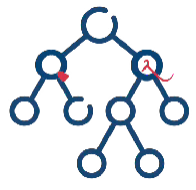
\includegraphics[height=0.9cm]{msca_logo.png}}%
  \end{center}
  \vspace{0.45cm}
  \begin{center}
    \begin{minipage}{0.1\textwidth}\centering
      \href{https://quantlet.com}{
\includegraphics[height=0.9cm]{ql_logo.png}}\end{minipage}%
    \begin{minipage}{0.78\textwidth}\centering
      {\Large\bfseries\usebeamercolor[fg]{title}\inserttitle}\par\vspace{0.25cm}
      {\large\usebeamercolor[fg]{title}\insertsubtitle}\end{minipage}%
    \begin{minipage}{0.1\textwidth}\centering
      \href{https://quantinar.com}{
\includegraphics[height=0.9cm]{qr_logo.png}}\end{minipage}
  \end{center}
  \vfill
  \hspace{0.4cm}{\bfseries\insertauthor}\par\vspace{0.12cm}
  \hspace{0.4cm}\begin{minipage}[t]{0.92\textwidth}\raggedright\footnotesize\insertinstitute\end{minipage}
  \par\vspace{0.4cm}}

% ---------------------------------------------------------------- lecture metadata
\newcommand{\nnshort}{}
\newcommand{\nnnb}{notebooks}
\newcommand{\nnrepo}{https://github.com/danpele/NEURAL_BIZ/tree/main}
% language-dependent labels (English default; \nnromanian switches to Romanian, call it before \nnlecture)
\newcommand{\txtcourse}{Neural Networks and Deep Learning}
\newcommand{\txtlecture}{Lecture}
\newcommand{\txtoutline}{Outline}
\newcommand{\txtintuition}{In one sentence:}
\newcommand{\txtjob}{In practice:}
\newcommand{\txttry}{Experiment yourself:}
\newcommand{\txtwhere}{where}
\newcommand{\txtsim}{SIMULATED DATA (teaching illustration)}
\newcommand{\txtnbsuffix}{}
\newcommand{\txtinstitute}{Bucharest University of Economic Studies (ASE), Department of Statistics and Econometrics\\
    Romanian Academy, Institute for Economic Forecasting (IPE)\\
    IDA Institute Digital Assets \textbullet\ AI4EFin \textbullet\ MSCA Digital Finance}
\newcommand{\nnromanian}{%
  \renewcommand{\txtcourse}{Rețele neuronale și deep learning}%
  \renewcommand{\txtlecture}{Cursul}%
  \renewcommand{\txtoutline}{Cuprins}%
  \renewcommand{\txtintuition}{Pe scurt:}%
  \renewcommand{\txtjob}{În practică:}%
  \renewcommand{\txttry}{Exercițiu practic:}%
  \renewcommand{\txtwhere}{unde}%
  \renewcommand{\txtsim}{DATE SIMULATE (doar pentru ilustrare)}%
  \renewcommand{\txtnbsuffix}{\string_ro}%
  \renewcommand{\txtinstitute}{Academia de Studii Economice din București (ASE), Departamentul de Statistică și Econometrie\\
    Academia Română, Institutul de Prognoză Economică (IPE)\\
    IDA Institute Digital Assets \textbullet\ AI4EFin \textbullet\ MSCA Digital Finance}}
\newcommand{\nnlecture}[2]{%
  \renewcommand{\nnshort}{\txtlecture\ #1}%
  \renewcommand{\nnnb}{notebooks/L#1\string_notebook\txtnbsuffix.ipynb}%
  \title[NN]{\txtcourse}%
  \subtitle{\txtlecture\ #1: #2}%
  \author{Prof.\ dr.\ Daniel Traian PELE}%
  \institute{\txtinstitute}%
  \date{}}

% ---------------------------------------------------------------- teaching blocks (one message per frame)
% \intuition{one plain sentence}  ->  formula with every symbol defined  ->  real-data example  ->  \manager{one line}
\newcommand{\intuition}[1]{\begin{itemize}\item {\color{MainBlue}\textbf{\txtintuition}}~#1\end{itemize}\vspace{0.6mm}}
\newcommand{\manager}[1]{\colorbox{Forest!10}{\parbox{\dimexpr\linewidth-2\fboxsep\relax}{\footnotesize
  \begin{itemize}\setlength{\itemsep}{0pt}\item \textbf{\color{Forest}\txtjob}~#1\end{itemize}}}}
% Experiment yourself: pointer to the matching notebook section
\newcommand{\tryit}[1]{{\scriptsize\href{\nnrepo/\nnnb}{%
  \raisebox{-0.15em}{
\includegraphics[height=0.85em]{ql_logo.png}}\,\textbf{\txttry}~\color{MainBlue}#1}}}
% bottom row: manager line (left) + experiment pointer (right), pinned to the bottom of the frame
\newcommand{\bottomrow}[2]{\par\vfill\noindent\begin{minipage}[b]{0.72\linewidth}#1\end{minipage}\hfill
  \begin{minipage}[b]{0.26\linewidth}\raggedleft #2\end{minipage}\par\vspace{0.5mm}}
\newcommand{\where}[1]{{\footnotesize\textbf{\txtwhere}~#1\par}}

% ---------------------------------------------------------------- helpers
% chart source line under a figure: \chartsource{Source ...; period ...}
\newcommand{\chartsource}[1]{\par\vspace{1pt}{\scriptsize\color{FooterGray}#1\par}}
% link to code: \quantlet{label}{path inside the repo}
\newcommand{\quantlet}[2]{\par\vspace{1pt}\hfill\href{\nnrepo/#2}{%
  \raisebox{-0.15em}{
\includegraphics[height=0.75em]{ql_logo.png}}\textcolor{MainBlue}{\scriptsize\ #1}}}
% inline Quantlet link for the bottom-right corner of a frame: \qlink{label}{path inside the repo}
\newcommand{\qlink}[2]{{\scriptsize\href{\nnrepo/#2}{\raisebox{-0.15em}{
\includegraphics[height=0.85em]{ql_logo.png}}\,\textcolor{MainBlue}{#1}}}}
\newcommand{\simlabel}{\colorbox{Crimson!12}{\scriptsize\bfseries\color{Crimson}\txtsim}}
\newcommand{\E}{\mathbb{E}}
\newcommand{\Var}{\operatorname{Var}}
\newcommand{\Cov}{\operatorname{Cov}}
\newcommand{\Corr}{\operatorname{Corr}}
\newcommand{\asinh}{\operatorname{asinh}}
\newcommand{\iid}{\overset{\text{i.i.d.}}{\sim}}
\newcommand{\EUR}{EUR}
% deep-learning notation (Bishop & Bishop, 2024): vectors bold lower case, matrices bold upper case
\newcommand{\R}{\mathbb{R}}
\newcommand{\vx}{\mathbf{x}}
\newcommand{\vy}{\mathbf{y}}
\newcommand{\vz}{\mathbf{z}}
\newcommand{\vh}{\mathbf{h}}
\newcommand{\vw}{\mathbf{w}}
\newcommand{\vb}{\mathbf{b}}
\newcommand{\mW}{\mathbf{W}}
\newcommand{\mX}{\mathbf{X}}
\newcommand{\btheta}{\boldsymbol{\theta}}
\newcommand{\loss}{\mathcal{L}}
\newcommand{\dataset}{\mathcal{D}}
\DeclareMathOperator*{\argmin}{arg\,min}
\DeclareMathOperator*{\argmax}{arg\,max}
\DeclareMathOperator{\softmax}{softmax}
\DeclareMathOperator{\ReLU}{ReLU}
\DeclareMathOperator{\sigm}{\sigma}

%   \nnlecture{k}{Lecture title}
% Logos live in lectures/common/logos/, charts in lectures/Lk/charts/.
% Do NOT add \hfuzz / \vfuzz / \hbadness here: overfull boxes must be fixed, not hidden.
% =============================================================================

\usetheme{default}
\setbeamersize{text margin left=7mm, text margin right=7mm}

% ---------------------------------------------------------------- packages
\usepackage[utf8]{inputenc}
\usepackage[T1]{fontenc}
\usepackage{lmodern}
\usepackage{amsmath, amssymb}
\usepackage{mathtools}
\usepackage{bm}
\usepackage{tikz}
\usetikzlibrary{arrows.meta, positioning, calc, shapes.misc}
\usepackage{booktabs}
\usepackage{array}
\usepackage{graphicx}
\usepackage{colortbl}
\usepackage{xcolor}
\usepackage{multicol}
\hypersetup{colorlinks=true, linkcolor=MainBlue, urlcolor=MainBlue, citecolor=MainBlue}
\graphicspath{{../common/logos/}}   % charts are included with their language folder: charts/en/, charts/ro/

% ---------------------------------------------------------------- colours
\definecolor{MainBlue}{RGB}{26, 58, 110}
\definecolor{IDAred}{RGB}{205, 0, 0}
\definecolor{DarkGray}{RGB}{51, 51, 51}
\definecolor{FooterGray}{RGB}{100, 100, 100}
\definecolor{BlockGray}{RGB}{236, 238, 242}
\definecolor{KeynoteGray}{RGB}{218, 218, 218}
\definecolor{Crimson}{RGB}{190, 40, 50}
\definecolor{Forest}{RGB}{30, 110, 50}
\definecolor{Bitter}{RGB}{214, 150, 20}
% chart palette (same hex values and order as lectures/common/nn_plot.py SERIES)
\definecolor{Ser1}{HTML}{2A78D6}
\definecolor{Ser2}{HTML}{EB6834}
\definecolor{Ser3}{HTML}{1BAF7A}
\definecolor{Ser4}{HTML}{EDA100}
\definecolor{Ser5}{HTML}{E87BA4}
\definecolor{Ser6}{HTML}{008300}
\definecolor{Ser7}{HTML}{6250D6}
\definecolor{Ser8}{HTML}{E34948}

\setbeamertemplate{background}{%
  \begin{tikzpicture}[remember picture, overlay]
    \shade[shading=axis, shading angle=315, top color=white, bottom color=KeynoteGray]
      (current page.south west) rectangle (current page.north east);
  \end{tikzpicture}}
\setbeamercolor{background canvas}{bg=}
\setbeamercolor{structure}{fg=MainBlue}
\setbeamercolor{normal text}{fg=DarkGray}
\setbeamercolor{title}{fg=IDAred}
\setbeamercolor{frametitle}{fg=IDAred, bg=}
\setbeamercolor{block title}{bg=MainBlue, fg=white}
\setbeamercolor{block body}{bg=BlockGray, fg=DarkGray}
\setbeamercolor{block title alerted}{bg=Crimson, fg=white}
\setbeamercolor{block body alerted}{bg=Crimson!7, fg=DarkGray}
\setbeamercolor{block title example}{bg=Forest, fg=white}
\setbeamercolor{block body example}{bg=Forest!7, fg=DarkGray}
\setbeamercolor{item}{fg=MainBlue}
\setbeamerfont{frametitle}{size=\large, series=\bfseries}
\setbeamerfont{block title}{size=\small, series=\bfseries}
\setbeamertemplate{blocks}[rounded][shadow=false]
\setbeamertemplate{itemize item}{\color{MainBlue}$\boxdot$}
\setbeamertemplate{itemize subitem}{\color{MainBlue}\scriptsize$\blacktriangleright$}
% compact two-level lists: level 1 = main point, level 2 = details (no text outside bullets)
\setbeamerfont{itemize/enumerate subbody}{size=\footnotesize}
\setlength{\leftmargini}{1.1em}
\setlength{\leftmarginii}{1.1em}
\setbeamertemplate{itemize/enumerate body begin}{\setlength{\topsep}{0pt}\setlength{\partopsep}{0pt}\setlength{\parskip}{0pt}}
\setbeamertemplate{itemize/enumerate subbody begin}{\setlength{\topsep}{0pt}\setlength{\partopsep}{0pt}\setlength{\itemsep}{0pt}\vspace{-0.4ex}}

\setbeamertemplate{enumerate item}{\color{MainBlue}\insertenumlabel.}
\setlength{\leftmargini}{1.3em}
\setlength{\leftmarginii}{1.2em}
\setbeamertemplate{navigation symbols}{}
\setbeamertemplate{section in toc}{\color{MainBlue}$\blacktriangleright$~\inserttocsection}
\setbeamertemplate{caption}{\raggedright\insertcaption\par}
% frame subtitle = precise citation line under the claim title (Weron style)
\setbeamerfont{framesubtitle}{size=\footnotesize}
\setbeamercolor{framesubtitle}{fg=FooterGray}
% outline that reappears at every section with the current section highlighted
\setbeamertemplate{section in toc shaded}[default][35]
\setbeamertemplate{subsection in toc shaded}[default][35]
\setbeamertemplate{subsection in toc}{\leavevmode\leftskip=2.2em\color{DarkGray}\small\inserttocsubsection\par}
\AtBeginSection[]{{\begin{frame}{\txtoutline}\vspace{2mm}\small
  \tableofcontents[currentsection,hideothersubsections]\end{frame}}}

% ---------------------------------------------------------------- head and foot
\setbeamertemplate{headline}{%
  \vskip10pt%
  \hbox to \paperwidth{\hskip0.5cm%
    {\small\color{FooterGray}\renewcommand{\hyperlink}[2]{##2}\insertsectionhead}%
    \hfill\textcolor{FooterGray}{\small\insertframenumber}\hskip0.5cm}%
  \vskip4pt{\color{FooterGray}\hrule height 0.4pt}}
% footer as in the other courses (MFM, SFM): course name on the left, small sparkline on the right
\setbeamertemplate{footline}{%
  {\color{FooterGray}\hrule height 0.4pt}\vskip4pt%
  \hbox to \paperwidth{\hskip0.5cm%
    \textcolor{FooterGray}{\small\txtcourse}%
    \hfill\raisebox{-0.1em}{\begin{tikzpicture}[x=0.08em, y=0.08em, line width=0.4pt]
      \draw[FooterGray] (0,3) -- (1,4) -- (2,3.5) -- (3,5) -- (4,4) -- (5,6) -- (6,5.5) -- (7,4) -- (8,5) -- (9,7) -- (10,6) -- (11,5) -- (12,6.5) -- (13,8) -- (14,7) -- (15,6) -- (16,7.5) -- (17,9) -- (18,8) -- (19,7) -- (20,8.5) -- (21,10) -- (22,9) -- (23,8) -- (24,9.5);
    \end{tikzpicture}}\hskip0.5cm}%
  \vskip6pt}

% ---------------------------------------------------------------- title page
\defbeamertemplate*{title page}{nn}[1][]{%
  \vspace{0.15cm}
  \begin{center}
    \href{https://www.ase.ro}{
\includegraphics[height=0.9cm]{ase_logo.png}}\hspace{0.3cm}%
    \href{https://ipe.ro/new}{
\includegraphics[height=0.9cm]{acad_logo.png}}\hspace{0.3cm}%
    \href{https://theida.net}{
\includegraphics[height=0.9cm]{ida_logo.png}}\hspace{0.3cm}%
    \href{https://blockchain-research-center.com}{
\includegraphics[height=0.9cm]{brc_logo.png}}\hspace{0.3cm}%
    \href{https://www.ai4efin.ase.ro}{
\includegraphics[height=0.9cm]{ai4efin_logo.png}}\hspace{0.3cm}%
    \href{https://www.digital-finance-msca.com}{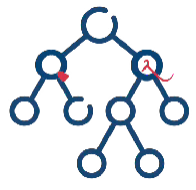
\includegraphics[height=0.9cm]{msca_logo.png}}%
  \end{center}
  \vspace{0.45cm}
  \begin{center}
    \begin{minipage}{0.1\textwidth}\centering
      \href{https://quantlet.com}{
\includegraphics[height=0.9cm]{ql_logo.png}}\end{minipage}%
    \begin{minipage}{0.78\textwidth}\centering
      {\Large\bfseries\usebeamercolor[fg]{title}\inserttitle}\par\vspace{0.25cm}
      {\large\usebeamercolor[fg]{title}\insertsubtitle}\end{minipage}%
    \begin{minipage}{0.1\textwidth}\centering
      \href{https://quantinar.com}{
\includegraphics[height=0.9cm]{qr_logo.png}}\end{minipage}
  \end{center}
  \vfill
  \hspace{0.4cm}{\bfseries\insertauthor}\par\vspace{0.12cm}
  \hspace{0.4cm}\begin{minipage}[t]{0.92\textwidth}\raggedright\footnotesize\insertinstitute\end{minipage}
  \par\vspace{0.4cm}}

% ---------------------------------------------------------------- lecture metadata
\newcommand{\nnshort}{}
\newcommand{\nnnb}{notebooks}
\newcommand{\nnrepo}{https://github.com/danpele/NEURAL_BIZ/tree/main}
% language-dependent labels (English default; \nnromanian switches to Romanian, call it before \nnlecture)
\newcommand{\txtcourse}{Neural Networks and Deep Learning}
\newcommand{\txtlecture}{Lecture}
\newcommand{\txtoutline}{Outline}
\newcommand{\txtintuition}{In one sentence:}
\newcommand{\txtjob}{In practice:}
\newcommand{\txttry}{Experiment yourself:}
\newcommand{\txtwhere}{where}
\newcommand{\txtsim}{SIMULATED DATA (teaching illustration)}
\newcommand{\txtnbsuffix}{}
\newcommand{\txtinstitute}{Bucharest University of Economic Studies (ASE), Department of Statistics and Econometrics\\
    Romanian Academy, Institute for Economic Forecasting (IPE)\\
    IDA Institute Digital Assets \textbullet\ AI4EFin \textbullet\ MSCA Digital Finance}
\newcommand{\nnromanian}{%
  \renewcommand{\txtcourse}{Rețele neuronale și deep learning}%
  \renewcommand{\txtlecture}{Cursul}%
  \renewcommand{\txtoutline}{Cuprins}%
  \renewcommand{\txtintuition}{Pe scurt:}%
  \renewcommand{\txtjob}{În practică:}%
  \renewcommand{\txttry}{Exercițiu practic:}%
  \renewcommand{\txtwhere}{unde}%
  \renewcommand{\txtsim}{DATE SIMULATE (doar pentru ilustrare)}%
  \renewcommand{\txtnbsuffix}{\string_ro}%
  \renewcommand{\txtinstitute}{Academia de Studii Economice din București (ASE), Departamentul de Statistică și Econometrie\\
    Academia Română, Institutul de Prognoză Economică (IPE)\\
    IDA Institute Digital Assets \textbullet\ AI4EFin \textbullet\ MSCA Digital Finance}}
\newcommand{\nnlecture}[2]{%
  \renewcommand{\nnshort}{\txtlecture\ #1}%
  \renewcommand{\nnnb}{notebooks/L#1\string_notebook\txtnbsuffix.ipynb}%
  \title[NN]{\txtcourse}%
  \subtitle{\txtlecture\ #1: #2}%
  \author{Prof.\ dr.\ Daniel Traian PELE}%
  \institute{\txtinstitute}%
  \date{}}

% ---------------------------------------------------------------- teaching blocks (one message per frame)
% \intuition{one plain sentence}  ->  formula with every symbol defined  ->  real-data example  ->  \manager{one line}
\newcommand{\intuition}[1]{\begin{itemize}\item {\color{MainBlue}\textbf{\txtintuition}}~#1\end{itemize}\vspace{0.6mm}}
\newcommand{\manager}[1]{\colorbox{Forest!10}{\parbox{\dimexpr\linewidth-2\fboxsep\relax}{\footnotesize
  \begin{itemize}\setlength{\itemsep}{0pt}\item \textbf{\color{Forest}\txtjob}~#1\end{itemize}}}}
% Experiment yourself: pointer to the matching notebook section
\newcommand{\tryit}[1]{{\scriptsize\href{\nnrepo/\nnnb}{%
  \raisebox{-0.15em}{
\includegraphics[height=0.85em]{ql_logo.png}}\,\textbf{\txttry}~\color{MainBlue}#1}}}
% bottom row: manager line (left) + experiment pointer (right), pinned to the bottom of the frame
\newcommand{\bottomrow}[2]{\par\vfill\noindent\begin{minipage}[b]{0.72\linewidth}#1\end{minipage}\hfill
  \begin{minipage}[b]{0.26\linewidth}\raggedleft #2\end{minipage}\par\vspace{0.5mm}}
\newcommand{\where}[1]{{\footnotesize\textbf{\txtwhere}~#1\par}}

% ---------------------------------------------------------------- helpers
% chart source line under a figure: \chartsource{Source ...; period ...}
\newcommand{\chartsource}[1]{\par\vspace{1pt}{\scriptsize\color{FooterGray}#1\par}}
% link to code: \quantlet{label}{path inside the repo}
\newcommand{\quantlet}[2]{\par\vspace{1pt}\hfill\href{\nnrepo/#2}{%
  \raisebox{-0.15em}{
\includegraphics[height=0.75em]{ql_logo.png}}\textcolor{MainBlue}{\scriptsize\ #1}}}
% inline Quantlet link for the bottom-right corner of a frame: \qlink{label}{path inside the repo}
\newcommand{\qlink}[2]{{\scriptsize\href{\nnrepo/#2}{\raisebox{-0.15em}{
\includegraphics[height=0.85em]{ql_logo.png}}\,\textcolor{MainBlue}{#1}}}}
\newcommand{\simlabel}{\colorbox{Crimson!12}{\scriptsize\bfseries\color{Crimson}\txtsim}}
\newcommand{\E}{\mathbb{E}}
\newcommand{\Var}{\operatorname{Var}}
\newcommand{\Cov}{\operatorname{Cov}}
\newcommand{\Corr}{\operatorname{Corr}}
\newcommand{\asinh}{\operatorname{asinh}}
\newcommand{\iid}{\overset{\text{i.i.d.}}{\sim}}
\newcommand{\EUR}{EUR}
% deep-learning notation (Bishop & Bishop, 2024): vectors bold lower case, matrices bold upper case
\newcommand{\R}{\mathbb{R}}
\newcommand{\vx}{\mathbf{x}}
\newcommand{\vy}{\mathbf{y}}
\newcommand{\vz}{\mathbf{z}}
\newcommand{\vh}{\mathbf{h}}
\newcommand{\vw}{\mathbf{w}}
\newcommand{\vb}{\mathbf{b}}
\newcommand{\mW}{\mathbf{W}}
\newcommand{\mX}{\mathbf{X}}
\newcommand{\btheta}{\boldsymbol{\theta}}
\newcommand{\loss}{\mathcal{L}}
\newcommand{\dataset}{\mathcal{D}}
\DeclareMathOperator*{\argmin}{arg\,min}
\DeclareMathOperator*{\argmax}{arg\,max}
\DeclareMathOperator{\softmax}{softmax}
\DeclareMathOperator{\ReLU}{ReLU}
\DeclareMathOperator{\sigm}{\sigma}

%   \nnlecture{k}{Lecture title}
% Logos live in lectures/common/logos/, charts in lectures/Lk/charts/.
% Do NOT add \hfuzz / \vfuzz / \hbadness here: overfull boxes must be fixed, not hidden.
% =============================================================================

\usetheme{default}
\setbeamersize{text margin left=7mm, text margin right=7mm}

% ---------------------------------------------------------------- packages
\usepackage[utf8]{inputenc}
\usepackage[T1]{fontenc}
\usepackage{lmodern}
\usepackage{amsmath, amssymb}
\usepackage{mathtools}
\usepackage{bm}
\usepackage{tikz}
\usetikzlibrary{arrows.meta, positioning, calc, shapes.misc}
\usepackage{booktabs}
\usepackage{array}
\usepackage{graphicx}
\usepackage{colortbl}
\usepackage{xcolor}
\usepackage{multicol}
\hypersetup{colorlinks=true, linkcolor=MainBlue, urlcolor=MainBlue, citecolor=MainBlue}
\graphicspath{{../common/logos/}}   % charts are included with their language folder: charts/en/, charts/ro/

% ---------------------------------------------------------------- colours
\definecolor{MainBlue}{RGB}{26, 58, 110}
\definecolor{IDAred}{RGB}{205, 0, 0}
\definecolor{DarkGray}{RGB}{51, 51, 51}
\definecolor{FooterGray}{RGB}{100, 100, 100}
\definecolor{BlockGray}{RGB}{236, 238, 242}
\definecolor{KeynoteGray}{RGB}{218, 218, 218}
\definecolor{Crimson}{RGB}{190, 40, 50}
\definecolor{Forest}{RGB}{30, 110, 50}
\definecolor{Bitter}{RGB}{214, 150, 20}
% chart palette (same hex values and order as lectures/common/nn_plot.py SERIES)
\definecolor{Ser1}{HTML}{2A78D6}
\definecolor{Ser2}{HTML}{EB6834}
\definecolor{Ser3}{HTML}{1BAF7A}
\definecolor{Ser4}{HTML}{EDA100}
\definecolor{Ser5}{HTML}{E87BA4}
\definecolor{Ser6}{HTML}{008300}
\definecolor{Ser7}{HTML}{6250D6}
\definecolor{Ser8}{HTML}{E34948}

\setbeamertemplate{background}{%
  \begin{tikzpicture}[remember picture, overlay]
    \shade[shading=axis, shading angle=315, top color=white, bottom color=KeynoteGray]
      (current page.south west) rectangle (current page.north east);
  \end{tikzpicture}}
\setbeamercolor{background canvas}{bg=}
\setbeamercolor{structure}{fg=MainBlue}
\setbeamercolor{normal text}{fg=DarkGray}
\setbeamercolor{title}{fg=IDAred}
\setbeamercolor{frametitle}{fg=IDAred, bg=}
\setbeamercolor{block title}{bg=MainBlue, fg=white}
\setbeamercolor{block body}{bg=BlockGray, fg=DarkGray}
\setbeamercolor{block title alerted}{bg=Crimson, fg=white}
\setbeamercolor{block body alerted}{bg=Crimson!7, fg=DarkGray}
\setbeamercolor{block title example}{bg=Forest, fg=white}
\setbeamercolor{block body example}{bg=Forest!7, fg=DarkGray}
\setbeamercolor{item}{fg=MainBlue}
\setbeamerfont{frametitle}{size=\large, series=\bfseries}
\setbeamerfont{block title}{size=\small, series=\bfseries}
\setbeamertemplate{blocks}[rounded][shadow=false]
\setbeamertemplate{itemize item}{\color{MainBlue}$\boxdot$}
\setbeamertemplate{itemize subitem}{\color{MainBlue}\scriptsize$\blacktriangleright$}
% compact two-level lists: level 1 = main point, level 2 = details (no text outside bullets)
\setbeamerfont{itemize/enumerate subbody}{size=\footnotesize}
\setlength{\leftmargini}{1.1em}
\setlength{\leftmarginii}{1.1em}
\setbeamertemplate{itemize/enumerate body begin}{\setlength{\topsep}{0pt}\setlength{\partopsep}{0pt}\setlength{\parskip}{0pt}}
\setbeamertemplate{itemize/enumerate subbody begin}{\setlength{\topsep}{0pt}\setlength{\partopsep}{0pt}\setlength{\itemsep}{0pt}\vspace{-0.4ex}}

\setbeamertemplate{enumerate item}{\color{MainBlue}\insertenumlabel.}
\setlength{\leftmargini}{1.3em}
\setlength{\leftmarginii}{1.2em}
\setbeamertemplate{navigation symbols}{}
\setbeamertemplate{section in toc}{\color{MainBlue}$\blacktriangleright$~\inserttocsection}
\setbeamertemplate{caption}{\raggedright\insertcaption\par}
% frame subtitle = precise citation line under the claim title (Weron style)
\setbeamerfont{framesubtitle}{size=\footnotesize}
\setbeamercolor{framesubtitle}{fg=FooterGray}
% outline that reappears at every section with the current section highlighted
\setbeamertemplate{section in toc shaded}[default][35]
\setbeamertemplate{subsection in toc shaded}[default][35]
\setbeamertemplate{subsection in toc}{\leavevmode\leftskip=2.2em\color{DarkGray}\small\inserttocsubsection\par}
\AtBeginSection[]{{\begin{frame}{\txtoutline}\vspace{2mm}\small
  \tableofcontents[currentsection,hideothersubsections]\end{frame}}}

% ---------------------------------------------------------------- head and foot
\setbeamertemplate{headline}{%
  \vskip10pt%
  \hbox to \paperwidth{\hskip0.5cm%
    {\small\color{FooterGray}\renewcommand{\hyperlink}[2]{##2}\insertsectionhead}%
    \hfill\textcolor{FooterGray}{\small\insertframenumber}\hskip0.5cm}%
  \vskip4pt{\color{FooterGray}\hrule height 0.4pt}}
% footer as in the other courses (MFM, SFM): course name on the left, small sparkline on the right
\setbeamertemplate{footline}{%
  {\color{FooterGray}\hrule height 0.4pt}\vskip4pt%
  \hbox to \paperwidth{\hskip0.5cm%
    \textcolor{FooterGray}{\small\txtcourse}%
    \hfill\raisebox{-0.1em}{\begin{tikzpicture}[x=0.08em, y=0.08em, line width=0.4pt]
      \draw[FooterGray] (0,3) -- (1,4) -- (2,3.5) -- (3,5) -- (4,4) -- (5,6) -- (6,5.5) -- (7,4) -- (8,5) -- (9,7) -- (10,6) -- (11,5) -- (12,6.5) -- (13,8) -- (14,7) -- (15,6) -- (16,7.5) -- (17,9) -- (18,8) -- (19,7) -- (20,8.5) -- (21,10) -- (22,9) -- (23,8) -- (24,9.5);
    \end{tikzpicture}}\hskip0.5cm}%
  \vskip6pt}

% ---------------------------------------------------------------- title page
\defbeamertemplate*{title page}{nn}[1][]{%
  \vspace{0.15cm}
  \begin{center}
    \href{https://www.ase.ro}{
\includegraphics[height=0.9cm]{ase_logo.png}}\hspace{0.3cm}%
    \href{https://ipe.ro/new}{
\includegraphics[height=0.9cm]{acad_logo.png}}\hspace{0.3cm}%
    \href{https://theida.net}{
\includegraphics[height=0.9cm]{ida_logo.png}}\hspace{0.3cm}%
    \href{https://blockchain-research-center.com}{
\includegraphics[height=0.9cm]{brc_logo.png}}\hspace{0.3cm}%
    \href{https://www.ai4efin.ase.ro}{
\includegraphics[height=0.9cm]{ai4efin_logo.png}}\hspace{0.3cm}%
    \href{https://www.digital-finance-msca.com}{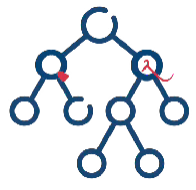
\includegraphics[height=0.9cm]{msca_logo.png}}%
  \end{center}
  \vspace{0.45cm}
  \begin{center}
    \begin{minipage}{0.1\textwidth}\centering
      \href{https://quantlet.com}{
\includegraphics[height=0.9cm]{ql_logo.png}}\end{minipage}%
    \begin{minipage}{0.78\textwidth}\centering
      {\Large\bfseries\usebeamercolor[fg]{title}\inserttitle}\par\vspace{0.25cm}
      {\large\usebeamercolor[fg]{title}\insertsubtitle}\end{minipage}%
    \begin{minipage}{0.1\textwidth}\centering
      \href{https://quantinar.com}{
\includegraphics[height=0.9cm]{qr_logo.png}}\end{minipage}
  \end{center}
  \vfill
  \hspace{0.4cm}{\bfseries\insertauthor}\par\vspace{0.12cm}
  \hspace{0.4cm}\begin{minipage}[t]{0.92\textwidth}\raggedright\footnotesize\insertinstitute\end{minipage}
  \par\vspace{0.4cm}}

% ---------------------------------------------------------------- lecture metadata
\newcommand{\nnshort}{}
\newcommand{\nnnb}{notebooks}
\newcommand{\nnrepo}{https://github.com/danpele/NEURAL_BIZ/tree/main}
% language-dependent labels (English default; \nnromanian switches to Romanian, call it before \nnlecture)
\newcommand{\txtcourse}{Neural Networks and Deep Learning}
\newcommand{\txtlecture}{Lecture}
\newcommand{\txtoutline}{Outline}
\newcommand{\txtintuition}{In one sentence:}
\newcommand{\txtjob}{In practice:}
\newcommand{\txttry}{Experiment yourself:}
\newcommand{\txtwhere}{where}
\newcommand{\txtsim}{SIMULATED DATA (teaching illustration)}
\newcommand{\txtnbsuffix}{}
\newcommand{\txtinstitute}{Bucharest University of Economic Studies (ASE), Department of Statistics and Econometrics\\
    Romanian Academy, Institute for Economic Forecasting (IPE)\\
    IDA Institute Digital Assets \textbullet\ AI4EFin \textbullet\ MSCA Digital Finance}
\newcommand{\nnromanian}{%
  \renewcommand{\txtcourse}{Rețele neuronale și deep learning}%
  \renewcommand{\txtlecture}{Cursul}%
  \renewcommand{\txtoutline}{Cuprins}%
  \renewcommand{\txtintuition}{Pe scurt:}%
  \renewcommand{\txtjob}{În practică:}%
  \renewcommand{\txttry}{Exercițiu practic:}%
  \renewcommand{\txtwhere}{unde}%
  \renewcommand{\txtsim}{DATE SIMULATE (doar pentru ilustrare)}%
  \renewcommand{\txtnbsuffix}{\string_ro}%
  \renewcommand{\txtinstitute}{Academia de Studii Economice din București (ASE), Departamentul de Statistică și Econometrie\\
    Academia Română, Institutul de Prognoză Economică (IPE)\\
    IDA Institute Digital Assets \textbullet\ AI4EFin \textbullet\ MSCA Digital Finance}}
\newcommand{\nnlecture}[2]{%
  \renewcommand{\nnshort}{\txtlecture\ #1}%
  \renewcommand{\nnnb}{notebooks/L#1\string_notebook\txtnbsuffix.ipynb}%
  \title[NN]{\txtcourse}%
  \subtitle{\txtlecture\ #1: #2}%
  \author{Prof.\ dr.\ Daniel Traian PELE}%
  \institute{\txtinstitute}%
  \date{}}

% ---------------------------------------------------------------- teaching blocks (one message per frame)
% \intuition{one plain sentence}  ->  formula with every symbol defined  ->  real-data example  ->  \manager{one line}
\newcommand{\intuition}[1]{\begin{itemize}\item {\color{MainBlue}\textbf{\txtintuition}}~#1\end{itemize}\vspace{0.6mm}}
\newcommand{\manager}[1]{\colorbox{Forest!10}{\parbox{\dimexpr\linewidth-2\fboxsep\relax}{\footnotesize
  \begin{itemize}\setlength{\itemsep}{0pt}\item \textbf{\color{Forest}\txtjob}~#1\end{itemize}}}}
% Experiment yourself: pointer to the matching notebook section
\newcommand{\tryit}[1]{{\scriptsize\href{\nnrepo/\nnnb}{%
  \raisebox{-0.15em}{
\includegraphics[height=0.85em]{ql_logo.png}}\,\textbf{\txttry}~\color{MainBlue}#1}}}
% bottom row: manager line (left) + experiment pointer (right), pinned to the bottom of the frame
\newcommand{\bottomrow}[2]{\par\vfill\noindent\begin{minipage}[b]{0.72\linewidth}#1\end{minipage}\hfill
  \begin{minipage}[b]{0.26\linewidth}\raggedleft #2\end{minipage}\par\vspace{0.5mm}}
\newcommand{\where}[1]{{\footnotesize\textbf{\txtwhere}~#1\par}}

% ---------------------------------------------------------------- helpers
% chart source line under a figure: \chartsource{Source ...; period ...}
\newcommand{\chartsource}[1]{\par\vspace{1pt}{\scriptsize\color{FooterGray}#1\par}}
% link to code: \quantlet{label}{path inside the repo}
\newcommand{\quantlet}[2]{\par\vspace{1pt}\hfill\href{\nnrepo/#2}{%
  \raisebox{-0.15em}{
\includegraphics[height=0.75em]{ql_logo.png}}\textcolor{MainBlue}{\scriptsize\ #1}}}
% inline Quantlet link for the bottom-right corner of a frame: \qlink{label}{path inside the repo}
\newcommand{\qlink}[2]{{\scriptsize\href{\nnrepo/#2}{\raisebox{-0.15em}{
\includegraphics[height=0.85em]{ql_logo.png}}\,\textcolor{MainBlue}{#1}}}}
\newcommand{\simlabel}{\colorbox{Crimson!12}{\scriptsize\bfseries\color{Crimson}\txtsim}}
\newcommand{\E}{\mathbb{E}}
\newcommand{\Var}{\operatorname{Var}}
\newcommand{\Cov}{\operatorname{Cov}}
\newcommand{\Corr}{\operatorname{Corr}}
\newcommand{\asinh}{\operatorname{asinh}}
\newcommand{\iid}{\overset{\text{i.i.d.}}{\sim}}
\newcommand{\EUR}{EUR}
% deep-learning notation (Bishop & Bishop, 2024): vectors bold lower case, matrices bold upper case
\newcommand{\R}{\mathbb{R}}
\newcommand{\vx}{\mathbf{x}}
\newcommand{\vy}{\mathbf{y}}
\newcommand{\vz}{\mathbf{z}}
\newcommand{\vh}{\mathbf{h}}
\newcommand{\vw}{\mathbf{w}}
\newcommand{\vb}{\mathbf{b}}
\newcommand{\mW}{\mathbf{W}}
\newcommand{\mX}{\mathbf{X}}
\newcommand{\btheta}{\boldsymbol{\theta}}
\newcommand{\loss}{\mathcal{L}}
\newcommand{\dataset}{\mathcal{D}}
\DeclareMathOperator*{\argmin}{arg\,min}
\DeclareMathOperator*{\argmax}{arg\,max}
\DeclareMathOperator{\softmax}{softmax}
\DeclareMathOperator{\ReLU}{ReLU}
\DeclareMathOperator{\sigm}{\sigma}

\usepackage[romanian]{babel}
\nnromanian
\nnlecture{7}{Atenția și transformerele}
\begin{document}
{\setbeamertemplate{headline}{}\setbeamertemplate{footline}{}
\begin{frame}\titlepage\end{frame}}
% END-FRONT-MATTER

\begin{frame}{Obiectivele cursului}
\small
\begin{itemize}\setlength{\itemsep}{5pt}
  \item De ce atenția a înlocuit recurența pentru text
    \begin{itemize}\setlength{\itemsep}{0pt}
      \item Un singur pas între oricare două cuvinte, calculat în paralel
    \end{itemize}
  \item Formulele atenției cu produs scalar scalat, ale atenției cu mai multe capete, ale codificării poziției și ale blocului transformer, cu toate simbolurile definite
  \item Compararea, pe tweet-uri financiare reale, a unui transformer mic antrenat de la zero, a unui model Bidirectional Encoder Representations from Transformers (BERT) preantrenat pentru finanțe (FinBERT) și a unui model de referință bazat pe frecvența termenului și inversul frecvenței în documente (TF-IDF)
  \item Citirea atentă a hărților de atenție
    \begin{itemize}\setlength{\itemsep}{0pt}
      \item Cînd preantrenarea, ajustarea fină sau un model simplu sînt alegerea potrivită pentru o firmă
    \end{itemize}
\end{itemize}
\end{frame}

% BEGIN-ABBR

\begin{frame}{Abrevieri}
\small
\vspace{-1mm}\begin{columns}[T,onlytextwidth]
\begin{column}{0.49\textwidth}{\scriptsize\renewcommand{\arraystretch}{0.96}\begin{tabular}{@{}>{\bfseries}l@{\ \ }p{0.74\linewidth}@{}}ASE & Academia de Studii Economice din București\\
BCE & Banca Centrală Europeană\\
BERT & Bidirectional Encoder Representations from Transformers (reprezentări bidirecționale ale codificatorului transformer)\\
CNN & rețea neuronală convoluțională\\
ES & pierderea așteptată în coadă (expected shortfall)\\
FFN & rețea directă aplicată fiecărei poziții (feed-forward)\\
FinBERT & BERT antrenat suplimentar pe texte financiare\\
GELU & unitate liniară cu eroare gaussiană (Gaussian error linear unit)\\
GPT & Generative Pre-trained Transformer (transformer generativ preantrenat)\\
IPE & Institutul de Prognoză Economică, Academia Română\\
LLM & model mare de limbaj\\\end{tabular}}\end{column}
\begin{column}{0.49\textwidth}{\scriptsize\renewcommand{\arraystretch}{0.96}\begin{tabular}{@{}>{\bfseries}l@{\ \ }p{0.74\linewidth}@{}}LN & normalizarea pe strat (layer normalisation)\\
LSTM & rețea cu memorie pe termen lung și scurt (long short-term memory)\\
MHA & atenția cu mai multe capete (multi-head attention)\\
MLM & modelarea limbajului cu cuvinte mascate (masked language modelling)\\
MPS & Metal Performance Shaders (interfața procesorului grafic Apple)\\
NLP & prelucrarea limbajului natural\\
ReLU & unitate liniară rectificată (rectified linear unit)\\
RNN & rețea neuronală recurentă\\
TF-IDF & frecvența termenului--inversul frecvenței în documente (TF-IDF)\\
VaR & valoarea la risc (Value-at-Risk)\\\end{tabular}}\end{column}
\end{columns}
\end{frame}

% END-ABBR


\section{De ce atenția}

\begin{frame}{Știrile financiare mișcă prețurile; mașinile trebuie să le citească repede}
\footnotesize
\intuition{Mii de titluri și postări sosesc în fiecare oră; o mesă de tranzacționare are nevoie de tonul lor în cîteva secunde, consecvent, pe aceeași scară.}
\begin{columns}[T,onlytextwidth]
\begin{column}{0.58\textwidth}
\[ \hat{\mathbf p}(x_{1:n})=\softmax\big(W_o\,\vh(x_{1:n})+\vb_o\big)\in\Delta^{3} \]{\footnotesize\begin{itemize}\setlength{\itemsep}{0pt}
  \item \textbf{\txtwhere}
    \begin{itemize}\setlength{\itemsep}{0pt}
      \item $x_{1:n}$ = tokenii unui text
      \item $\vh$ = o reprezentare de dimensiune fixă a textului
      \item $\Delta^3$ = probabilitățile pentru negativ (bearish), pozitiv (bullish), neutru
      \item Tot cursul este despre cum se calculează $\vh$.
    \end{itemize}
\end{itemize}\par}
\end{column}
\begin{column}{0.39\textwidth}
\begin{itemize}\setlength{\itemsep}{3pt}
  \item \textbf{Datele noastre}
    \begin{itemize}\setlength{\itemsep}{0pt}
      \item 9\,543 de tweet-uri financiare etichetate pentru antrenare, 2\,388 pentru test
      \item Test: 14{,}5\,\% negative, 19{,}9\,\% pozitive, 65{,}6\,\% neutre
    \end{itemize}
  \item \textbf{Dovezi}
    \begin{itemize}\setlength{\itemsep}{0pt}
      \item Pesimismul din presă anticipează randamentele și volumul din ziua următoare (Tetlock, 2007)
    \end{itemize}
\end{itemize}
\end{column}
\end{columns}
\par\vfill\manager{un model de sentiment este un instrument de măsură: trebuie să fie precis pe știrile negative rare, nu doar în medie.}\par\vspace{0.5mm}
\par\vfill\noindent{\scriptsize\color{FooterGray}(Tetlock, 2007; Malo et al., 2014)}\par\vspace{0.5mm}
\end{frame}

\begin{frame}{Rețelele recurente citesc cuvînt cu cuvînt și uită}
\footnotesize
\intuition{O rețea recurentă comprimă tot ce a citit pînă acum într-un singur vector de stare, actualizat token cu token.}
\begin{columns}[T,onlytextwidth]
\begin{column}{0.58\textwidth}
\[ \vh_t=\phi\big(W_h\vh_{t-1}+W_x\vx_t+\vb\big),\qquad \frac{\partial\vh_n}{\partial\vh_1}=\prod_{t=2}^{n}\frac{\partial\vh_t}{\partial\vh_{t-1}} \]{\footnotesize\begin{itemize}\setlength{\itemsep}{0pt}
  \item \textbf{\txtwhere}
    \begin{itemize}\setlength{\itemsep}{0pt}
      \item $\vx_t$ = reprezentarea tokenului $t$
      \item $\vh_t$ = starea
      \item $\phi$ = tanh
      \item Produsul a $n-1$ matrice jacobiene scade sau explodează odată cu distanța dintre cuvinte.
    \end{itemize}
\end{itemize}\par}
\end{column}
\begin{column}{0.39\textwidth}
\begin{itemize}\setlength{\itemsep}{3pt}
  \item \textbf{Două costuri}
    \begin{itemize}\setlength{\itemsep}{0pt}
      \item Drumul dintre cuvintele $i$ și $j$: $|i-j|$ pași, deci legăturile lungi se estompează
      \item $n$ pași succesivi: nicio paralelizare pe propoziție
    \end{itemize}
  \item \textbf{Porțile ajută, dar nu vindecă}
    \begin{itemize}\setlength{\itemsep}{0pt}
      \item Rețeaua cu memorie pe termen lung și scurt (LSTM) din cursul 5 atenuează, dar păstrează drumul secvențial
    \end{itemize}
\end{itemize}
\end{column}
\end{columns}
\par\vfill\manager{în ``profitul a scăzut, dar prognoza a fost majorată'', verdictul depinde de un cuvînt aflat departe de subiect.}\par\vspace{0.5mm}
\par\vfill\noindent{\scriptsize\color{FooterGray}(Bahdanau, Cho \& Bengio, 2015; Bishop \& Bishop, 2024, sec.\ 12.1)}\par\vspace{0.5mm}
\end{frame}

\begin{frame}{Tweet-urile sînt scurte; discursurile băncilor centrale depășesc mult fereastra de 512 tokeni}
\small
\begin{center}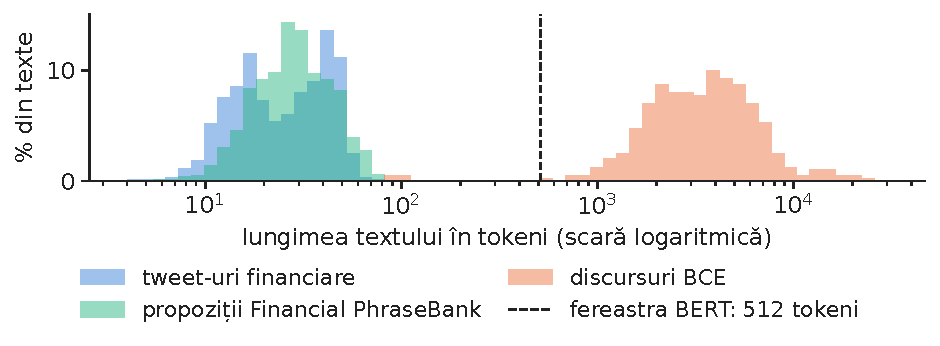
\includegraphics[width=\textwidth,height=0.314\textheight,keepaspectratio]{charts/ro/context_lengths.pdf}\end{center}\vspace{-3mm}
\chartsource{Sursa: Twitter financial news (zeroshot); Malo et al. (2014); discursurile Băncii Centrale Europene; tokenizatorul modelului ProsusAI. Date: tweet-uri financiare; Financial PhraseBank; discursurile Băncii Centrale Europene 8 ianuarie 2022 - 30 octombrie 2026.}
\vspace{0.5mm}
\begin{itemize}\setlength{\itemsep}{0pt}
  \item \textbf{Lungimea mediană în tokeni}: tweet-uri 25, propoziții Financial PhraseBank 28, discursuri ale Băncii Centrale Europene (BCE) 3\,338
  \item \textbf{Limita de context}: 98{,}8\,\% dintre cele 400 de discursuri depășesc 512 tokeni
    \begin{itemize}\setlength{\itemsep}{0pt}
      \item Doar 0{,}19\,\% dintre tweet-uri depășesc 64
    \end{itemize}
\end{itemize}
\par\vfill\manager{potriviți modelul cu lungimea textului: un tweet încape în orice transformer, un discurs cere împărțire sau un model cu context lung.}\par\vspace{0.5mm}
\par\vfill\noindent{\scriptsize\color{FooterGray}}\hfill\qlink{NN\_L7\_context\_lengths}{Quantlets/L7/NN_L7_context_lengths}\par\vspace{0.5mm}
\end{frame}


\section{Mecanismul atenției}

\begin{frame}{Atenția este o căutare aproximativă într-un dicționar}
\footnotesize
\intuition{Fiecare cuvînt pune o întrebare (query), fiecare cuvînt oferă o etichetă (key) și un conținut (value); răspunsul este media valorilor, ponderată după potrivirea cheilor cu întrebarea.}
\begin{columns}[T,onlytextwidth]
\begin{column}{0.58\textwidth}
\[ \vy_i=\sum_{j=1}^{n}a_{ij}\,\mathbf v_j,\qquad a_{ij}=\frac{\exp\big(\mathbf q_i^{\top}\mathbf k_j/\sqrt{d_k}\big)}{\sum_{l=1}^{n}\exp\big(\mathbf q_i^{\top}\mathbf k_l/\sqrt{d_k}\big)} \]\[ \mathbf q_i=W_Q^{\top}\vx_i,\quad \mathbf k_j=W_K^{\top}\vx_j,\quad \mathbf v_j=W_V^{\top}\vx_j \]{\footnotesize\begin{itemize}\setlength{\itemsep}{0pt}
  \item \textbf{\txtwhere}
    \begin{itemize}\setlength{\itemsep}{0pt}
      \item $\vx_i\in\R^{d}$ = reprezentarea tokenului
      \item $W_Q,W_K\in\R^{d\times d_k}$, $W_V\in\R^{d\times d_v}$ = proiecții învățate
      \item $a_{ij}\ge0$, $\sum_j a_{ij}=1$: o distribuție de probabilitate pe cuvinte.
    \end{itemize}
\end{itemize}\par}
\end{column}
\begin{column}{0.39\textwidth}
\begin{itemize}\setlength{\itemsep}{3pt}
  \item \textbf{Căutarea exactă}
    \begin{itemize}\setlength{\itemsep}{0pt}
      \item Un dicționar întoarce valoarea singurei chei potrivite
    \end{itemize}
  \item \textbf{Căutarea aproximativă}
    \begin{itemize}\setlength{\itemsep}{0pt}
      \item Atenția întoarce un amestec al tuturor valorilor: derivabil, deci $W_Q,W_K,W_V$ se învață
      \item Un singur pas între oricare două cuvinte, oricare ar fi distanța
    \end{itemize}
\end{itemize}
\end{column}
\end{columns}
\par\vfill\manager{fiecare cuvînt de ieșire este un amestec care ține cont de context: ``prognoza'' poate împrumuta sens de la ``majorată'', aflat zece cuvinte mai departe.}\par\vspace{0.5mm}
\par\vfill\noindent{\scriptsize\color{FooterGray}(Vaswani et al., 2017; Bishop \& Bishop, 2024, sec.\ 12.1)}\hfill\tryit{notebook, secțiunea 2}\par\vspace{0.5mm}
\end{frame}

\begin{frame}{În formă matriceală: o singură înmulțire calculează atenția pentru toate cuvintele}
\footnotesize
\intuition{Așezînd întrebările, cheile și valorile în matrice, atenția devine două produse de matrice și un softmax pe rînduri.}
\begin{columns}[T,onlytextwidth]
\begin{column}{0.58\textwidth}
\[ \operatorname{Attention}(Q,K,V)=\softmax\Big(\frac{QK^{\top}}{\sqrt{d_k}}+\mathbf M\Big)V \]\[ Q=XW_Q,\quad K=XW_K,\quad V=XW_V \]{\footnotesize\begin{itemize}\setlength{\itemsep}{0pt}
  \item \textbf{\txtwhere}
    \begin{itemize}\setlength{\itemsep}{0pt}
      \item $X\in\R^{n\times d}$ = cele $n$ reprezentări ale tokenilor
      \item $QK^{\top}\in\R^{n\times n}$ = toate scorurile perechilor
      \item $\mathbf M$ = masca, $0$ pentru perechile permise și $-\infty$ pentru completare (sau pentru tokenii viitori, într-un decodor).
    \end{itemize}
\end{itemize}\par}
\end{column}
\begin{column}{0.39\textwidth}
\begin{itemize}\setlength{\itemsep}{3pt}
  \item \textbf{Costul pe strat}
    \begin{itemize}\setlength{\itemsep}{0pt}
      \item $O(n^2d)$ operații și memorie $O(n^2)$
      \item Un discurs median costă de circa 17\,828 de ori mai mult decît un tweet median
    \end{itemize}
  \item \textbf{Paralel}
    \begin{itemize}\setlength{\itemsep}{0pt}
      \item Fără buclă pe poziții: procesoarele grafice înmulțesc toată propoziția deodată
    \end{itemize}
\end{itemize}
\end{column}
\end{columns}
\par\vfill\manager{termenul $n^2$ explică de ce ferestrele de context sînt limitate și rapoartele lungi trebuie tăiate în bucăți.}\par\vspace{0.5mm}
\par\vfill\noindent{\scriptsize\color{FooterGray}(Vaswani et al., 2017)}\hfill\tryit{notebook, secțiunea 2}\par\vspace{0.5mm}
\end{frame}

\begin{frame}{De ce împărțim la $\sqrt{d_k}$: ferim softmax-ul de saturație}
\footnotesize
\intuition{Produsele scalare ale unor vectori aleatori lungi cresc odată cu lungimea lor; fără scalare, softmax-ul devine one-hot și gradientul dispare.}
\begin{columns}[T,onlytextwidth]
\begin{column}{0.58\textwidth}
\[ q_l,k_l\iid(0,1)\ \Rightarrow\ \E[\mathbf q^{\top}\mathbf k]=0,\quad \Var(\mathbf q^{\top}\mathbf k)=\sum_{l=1}^{d_k}\Var(q_lk_l)=d_k \]\[ \Var\big(\mathbf q^{\top}\mathbf k/\sqrt{d_k}\big)=1\quad\text{pentru orice}\ d_k \]{\footnotesize\begin{itemize}\setlength{\itemsep}{0pt}
  \item \textbf{\txtwhere}
    \begin{itemize}\setlength{\itemsep}{0pt}
      \item $d_k$ = dimensiunea întrebărilor și cheilor (64 pe cap în BERT)
      \item Cu scoruri de varianță unu, softmax-ul își împarte masa, iar jacobianul $\operatorname{diag}(\mathbf a)-\mathbf a\mathbf a^{\top}$ nu se apropie de zero.
    \end{itemize}
\end{itemize}\par}
\end{column}
\begin{column}{0.39\textwidth}
\begin{itemize}\setlength{\itemsep}{3pt}
  \item \textbf{Fără scalare}
    \begin{itemize}\setlength{\itemsep}{0pt}
      \item Cu $d_k=64$ scorurile au abaterea standard 8, deci un singur cuvînt ia aproape toată ponderea
    \end{itemize}
  \item \textbf{Interpretare ca temperatură}
    \begin{itemize}\setlength{\itemsep}{0pt}
      \item $\sqrt{d_k}$ este o temperatură fixă care păstrează atenția difuză la inițializare
    \end{itemize}
\end{itemize}
\end{column}
\end{columns}
\par\vfill\manager{o constantă de proiectare, nu un parametru de calibrat: datorită ei se pot antrena stive adînci de straturi de atenție.}\par\vspace{0.5mm}
\par\vfill\noindent{\scriptsize\color{FooterGray}(Vaswani et al., 2017)}\par\vspace{0.5mm}
\end{frame}

\begin{frame}{Mai multe capete caută simultan mai multe relații}
\footnotesize
\intuition{Un cap mediază un singur tip de relație; mai multe capete, cu proiecții mai mici, surprind în paralel sintaxa, negația și entitățile.}
\begin{columns}[T,onlytextwidth]
\begin{column}{0.58\textwidth}
\[ \operatorname{MHA}(X)=\big[\mathbf H_1\,\|\,\cdots\,\|\,\mathbf H_h\big]W_O \]\[ \mathbf H_m=\operatorname{Attention}(XW_Q^{m},XW_K^{m},XW_V^{m}) \]{\footnotesize\begin{itemize}\setlength{\itemsep}{0pt}
  \item \textbf{\txtwhere}
    \begin{itemize}\setlength{\itemsep}{0pt}
      \item $h$ = numărul de capete
      \item $W_Q^m,W_K^m,W_V^m\in\R^{d\times d/h}$
      \item $\|$ = concatenare
      \item $W_O\in\R^{d\times d}$
      \item Parametri: $4d^2$ (plus termenii liberi), ca la un singur cap mare.
    \end{itemize}
\end{itemize}\par}
\end{column}
\begin{column}{0.39\textwidth}
\begin{itemize}\setlength{\itemsep}{3pt}
  \item \textbf{BERT-base}
    \begin{itemize}\setlength{\itemsep}{0pt}
      \item 12 straturi $\times$ 12 capete, $d=$ 768, $d/h=$ 64
    \end{itemize}
  \item \textbf{Transformerul nostru mic}
    \begin{itemize}\setlength{\itemsep}{0pt}
      \item 2 straturi $\times$ 4 capete, $d=64$, $d/h=16$
    \end{itemize}
\end{itemize}
\end{column}
\end{columns}
\par\vfill\manager{capetele sînt specialiști ieftini: același cost ca un singur cap, mai multe tipuri de context pe strat.}\par\vspace{0.5mm}
\par\vfill\noindent{\scriptsize\color{FooterGray}(Vaswani et al., 2017; Clark et al., 2019)}\hfill\tryit{notebook, secțiunea 2}\par\vspace{0.5mm}
\end{frame}

\begin{frame}{La ce este atent FinBERT într-un tweet negativ real}
\small
\begin{center}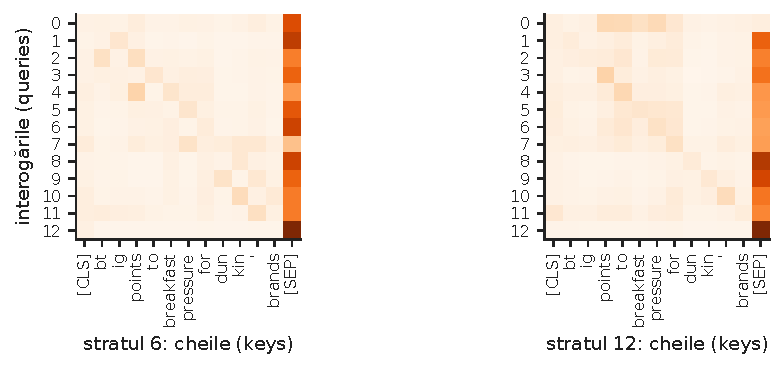
\includegraphics[width=\textwidth,height=0.520\textheight,keepaspectratio]{charts/ro/attention_example.pdf}\end{center}\vspace{-3mm}
\chartsource{Sursa: Seturile Twitter financial news (Hugging Face, zeroshot). Date: un tweet de test; FinBERT preantrenat, atenția mediată pe 12 capete.}
\vspace{0.5mm}
\begin{itemize}\setlength{\itemsep}{0pt}
  \item \textbf{Tweet-ul} (setul de test, etichetă negativă): ``BTIG points to breakfast pressure for Dunkin' Brands''
    \begin{itemize}\setlength{\itemsep}{0pt}
      \item FinBERT preantrenat îi dă doar 7{,}3\,\% probabilitate de a fi negativ: tonul negativ este implicit
    \end{itemize}
  \item \textbf{Stratul 6}: tokenul [CLS] pune 5{,}7\,\% din atenție pe ``points''
    \begin{itemize}\setlength{\itemsep}{0pt}
      \item În stratul 12, cea mai mare parte a ponderii merge spre tokenii separatori
    \end{itemize}
\end{itemize}
\par\vfill\noindent{\scriptsize\color{FooterGray}(calcule proprii; media pe cele 12 capete)}\hfill\qlink{NN\_L7\_attention\_example}{Quantlets/L7/NN_L7_attention_example}\par\vspace{0.5mm}
\end{frame}

\begin{frame}{De la un strat la altul, atenția se concentrează și se oprește pe tokenii separatori}
\small
\begin{center}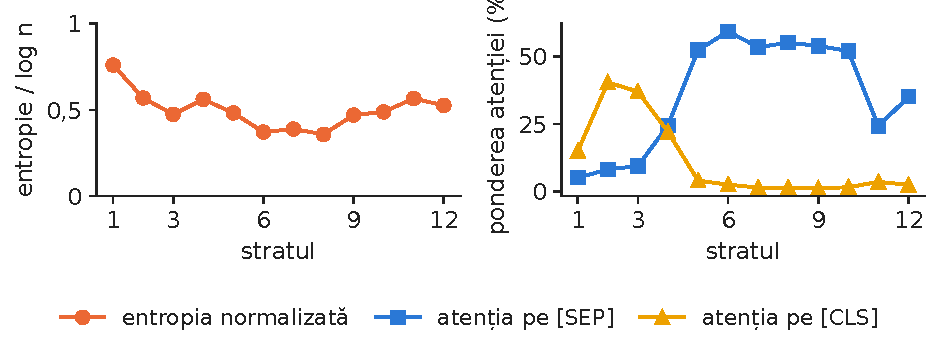
\includegraphics[width=\textwidth,height=0.456\textheight,keepaspectratio]{charts/ro/attention_entropy.pdf}\end{center}\vspace{-3mm}
\chartsource{Sursa: Seturile Twitter financial news (Hugging Face, zeroshot). Date: 500 de tweet-uri de test; FinBERT preantrenat.}
\vspace{0.5mm}
\begin{itemize}\setlength{\itemsep}{0pt}
  \item \textbf{Entropia} rîndurilor de atenție, împărțită la $\log n$: 0{,}76 în stratul 1, minimul 0{,}36 în stratul 8 (1 = uniformă)
  \item \textbf{[SEP] ca destinație implicită}: pînă la 59{,}3\,\% din toată atenția (stratul 6) merge spre separator, o operație nulă pe care un cap o folosește cînd nu are nimic de adăugat
\end{itemize}
\par\vfill\noindent{\scriptsize\color{FooterGray}(calcule proprii, 500 de tweet-uri de test; Clark et al., 2019)}\hfill\qlink{NN\_L7\_attention\_entropy}{Quantlets/L7/NN_L7_attention_entropy}\par\vspace{0.5mm}
\end{frame}

\begin{frame}{Ponderile de atenție sînt un indiciu, nu o explicație}
\footnotesize
\intuition{Unde se uită un cap nu este același lucru cu motivul deciziei: valorile, straturile următoare și clasificatorul transformă tot ce selectează atenția.}
\begin{columns}[T,onlytextwidth]
\begin{column}{0.58\textwidth}
\[ \vh_i^{(l+1)}=\vh_i^{(l)}+\sum_{m=1}^{h}\sum_{j}a_{ij}^{(l,m)}\,W_O^{m\top}W_V^{m\top}\vh_j^{(l)}+\dots \]{\footnotesize\begin{itemize}\setlength{\itemsep}{0pt}
  \item \textbf{\txtwhere}
    \begin{itemize}\setlength{\itemsep}{0pt}
      \item Contribuția cuvîntului $j$ este $a_{ij}$ înmulțit cu un vector de valori a cărui normă poate fi mare sau mică
      \item Fluxul rezidual $\vh_i^{(l)}$ duce informație pe care atenția nu o atinge.
    \end{itemize}
\end{itemize}\par}
\end{column}
\begin{column}{0.39\textwidth}
\begin{itemize}\setlength{\itemsep}{3pt}
  \item \textbf{Dovezi}
    \begin{itemize}\setlength{\itemsep}{0pt}
      \item Hărți de atenție diferite pot da aceeași predicție (Jain \& Wallace, 2019)
      \item Atenția mare pe [SEP] nu poartă aproape nicio informație (Clark et al., 2019)
    \end{itemize}
  \item \textbf{Instrumente mai bune}
    \begin{itemize}\setlength{\itemsep}{0pt}
      \item Atribuiri bazate pe gradient și teste de ocluzie (cursul 11)
    \end{itemize}
\end{itemize}
\end{column}
\end{columns}
\par\vfill\manager{nu prezentați niciodată unui supraveghetor o hartă de atenție drept ``motivul'' unei decizii.}\par\vspace{0.5mm}
\par\vfill\noindent{\scriptsize\color{FooterGray}(Jain \& Wallace, 2019; Clark et al., 2019)}\par\vspace{0.5mm}
\end{frame}


\section{Arhitectura transformer}

\begin{frame}{Atenția ignoră ordinea; codificarea poziției o readuce}
\small
\begin{center}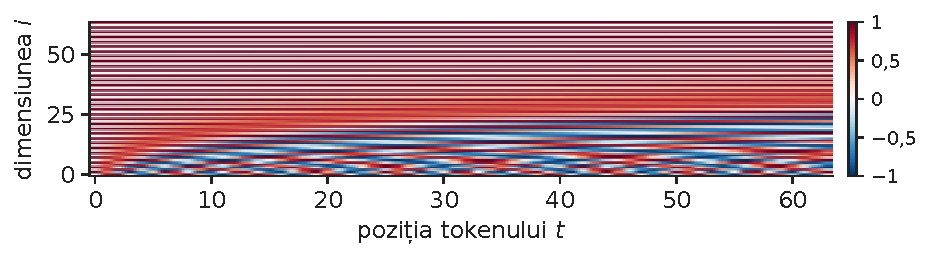
\includegraphics[width=\textwidth,height=0.480\textheight,keepaspectratio]{charts/ro/positional_encoding.pdf}\end{center}\vspace{-3mm}
\chartsource{Sursa: Vaswani et al. (2017), formula sinusoidală. Date: ilustrarea mecanismului, $d=64$, 64 de poziții.}
\vspace{0.5mm}
\begin{itemize}\setlength{\itemsep}{0pt}
  \item \textbf{Formula}: $p_{t,2i}=\sin(t/10000^{2i/d})$, $p_{t,2i+1}=\cos(t/10000^{2i/d})$, adunată la reprezentarea tokenului
    \begin{itemize}\setlength{\itemsep}{0pt}
      \item Dimensiunile mici se schimbă repede, cele mari încet
    \end{itemize}
  \item \textbf{De ce}: auto-atenția este echivariantă la permutări
    \begin{itemize}\setlength{\itemsep}{0pt}
      \item Fără poziții, ``dobînzile scad, acțiunile cresc'' este totuna cu ``acțiunile scad, dobînzile cresc''
    \end{itemize}
\end{itemize}
\par\vfill\noindent{\scriptsize\color{FooterGray}\simlabel\ (Vaswani et al., 2017)}\hfill\qlink{NN\_L7\_positional\_encoding}{Quantlets/L7/NN_L7_positional_encoding}\par\vspace{0.5mm}
\end{frame}

\begin{frame}{Un bloc transformer: atenție, rețea directă, conexiuni reziduale, normalizare}
\footnotesize
\intuition{Atenția amestecă informația între cuvinte; o rețea mică cu două straturi transformă apoi fiecare cuvînt separat; conexiunile reziduale și normalizarea pe strat stabilizează antrenarea.}
\begin{columns}[T,onlytextwidth]
\begin{column}{0.58\textwidth}
\[ Z=X+\operatorname{MHA}\big(\operatorname{LN}(X)\big),\qquad X'=Z+\operatorname{FFN}\big(\operatorname{LN}(Z)\big) \]\[ \operatorname{FFN}(\vz)=W_2\,\operatorname{GELU}(W_1\vz+\vb_1)+\vb_2,\quad \operatorname{LN}(\vz)=\boldsymbol\gamma\odot\frac{\vz-\mu_{\vz}}{\sigma_{\vz}}+\boldsymbol\beta \]{\footnotesize\begin{itemize}\setlength{\itemsep}{0pt}
  \item \textbf{\txtwhere}
    \begin{itemize}\setlength{\itemsep}{0pt}
      \item Varianta cu normalizare înainte
      \item Rețeaua directă aplicată fiecărei poziții (FFN), $W_1\in\R^{4d\times d}$
      \item Unitatea liniară cu eroare gaussiană (GELU) sau unitatea liniară rectificată (ReLU)
      \item Normalizarea pe strat (LN), pe cele $d$ variabile ale unui token
      \item Parametri pe bloc $\approx12d^2$.
    \end{itemize}
\end{itemize}\par}
\end{column}
\begin{column}{0.39\textwidth}
\begin{itemize}\setlength{\itemsep}{3pt}
  \item \textbf{Conexiunile reziduale}
    \begin{itemize}\setlength{\itemsep}{0pt}
      \item Gradientul ajunge direct la primele straturi (cursul 4)
    \end{itemize}
  \item \textbf{Blocul nostru}
    \begin{itemize}\setlength{\itemsep}{0pt}
      \item $d=64$, lățimea FFN 128, dropout 0,1; 2 blocuri: 67\,139 de parametri în afara reprezentărilor
    \end{itemize}
\end{itemize}
\end{column}
\end{columns}
\par\vfill\manager{cei mai mulți parametri ai unui transformer se află în straturile directe, nu în atenție.}\par\vspace{0.5mm}
\par\vfill\noindent{\scriptsize\color{FooterGray}(Vaswani et al., 2017; Ba, Kiros \& Hinton, 2016)}\hfill\tryit{notebook, secțiunea 3}\par\vspace{0.5mm}
\end{frame}

\begin{frame}{Codificatoarele citesc, decodoarele scriu: două sarcini de preantrenare}
\footnotesize
\intuition{Același bloc devine cititor sau scriitor în funcție de mască și de sarcina de preantrenare.}
\begin{columns}[T,onlytextwidth]
\begin{column}{0.58\textwidth}
\[ \loss_{\text{MLM}}=-\sum_{i\in\mathcal M}\log p_{\btheta}\big(x_i\mid x_{\setminus\mathcal M}\big) \]\[ \loss_{\text{LM}}=-\sum_{t=1}^{n}\log p_{\btheta}\big(x_t\mid x_{<t}\big) \]{\footnotesize\begin{itemize}\setlength{\itemsep}{0pt}
  \item \textbf{\txtwhere}
    \begin{itemize}\setlength{\itemsep}{0pt}
      \item $\mathcal M$ = 15\,\% dintre poziții, mascate aleator: modelarea limbajului cu cuvinte mascate (MLM), bidirecțională
      \item Dreapta: prezicerea tokenului următor, cu mască cauzală, $M_{ij}=-\infty$ pentru $j>i$.
    \end{itemize}
\end{itemize}\par}
\end{column}
\begin{column}{0.39\textwidth}
\begin{itemize}\setlength{\itemsep}{3pt}
  \item \textbf{Doar codificator}
    \begin{itemize}\setlength{\itemsep}{0pt}
      \item Bidirectional Encoder Representations from Transformers (BERT): clasificare, extragere de informații
    \end{itemize}
  \item \textbf{Doar decodor}
    \begin{itemize}\setlength{\itemsep}{0pt}
      \item Generative Pre-trained Transformer (GPT): generare de text, modelele mari de limbaj (LLM) de azi
    \end{itemize}
\end{itemize}
\end{column}
\end{columns}
\par\vfill\manager{pentru etichetarea textelor folosiți un codificator
    \begin{itemize}\setlength{\itemsep}{0pt}
      \item Pentru redactarea rapoartelor, un decodor (cursul 12).
    \end{itemize}}\par\vspace{0.5mm}
\par\vfill\noindent{\scriptsize\color{FooterGray}(Devlin et al., 2019; Radford et al., 2018)}\par\vspace{0.5mm}
\end{frame}

\begin{frame}{Textul devine numere prin tokeni de subcuvinte}
\footnotesize
\intuition{Un vocabular fix de bucăți de cuvinte acoperă orice cuvînt, inclusiv simbolurile bursiere și numele noi de firme, împărțind cuvintele rare în bucăți frecvente.}
\begin{columns}[T,onlytextwidth]
\begin{column}{0.58\textwidth}
\[ x_{1:n}=\big[\texttt{[CLS]},w_1,\dots,w_{n-2},\texttt{[SEP]}\big],\qquad \vx_t=E[x_t]+\mathbf p_t+\mathbf s_t \]{\footnotesize\begin{itemize}\setlength{\itemsep}{0pt}
  \item \textbf{\txtwhere}
    \begin{itemize}\setlength{\itemsep}{0pt}
      \item $E\in\R^{|\mathcal V|\times d}$ = tabelul reprezentărilor
      \item $\mathbf p_t$ = poziția, $\mathbf s_t$ = segmentul
      \item [CLS] rezumă textul, [SEP] îl închide
      \item Vocabularul WordPiece al FinBERT: $|\mathcal V|=$ 30\,522.
    \end{itemize}
\end{itemize}\par}
\end{column}
\begin{column}{0.39\textwidth}
\begin{itemize}\setlength{\itemsep}{3pt}
  \item \textbf{Tweet-urile noastre}
    \begin{itemize}\setlength{\itemsep}{0pt}
      \item Mediana 25 de tokeni, percentila 99 este 57, maximul 82
      \item Tăiem la 64 de tokeni: 0{,}19\,\% dintre tweet-uri pierd cîțiva tokeni
    \end{itemize}
  \item \textbf{Reprezentările domină modelele mici}
    \begin{itemize}\setlength{\itemsep}{0pt}
      \item Transformerul mic: 2\,020\,547 de parametri, dintre care 67\,139 în afara tabelului
    \end{itemize}
\end{itemize}
\end{column}
\end{columns}
\par\vfill\manager{verificați cum împarte tokenizatorul simbolurile bursiere și numele produselor înainte de a avea încredere în model.}\par\vspace{0.5mm}
\par\vfill\noindent{\scriptsize\color{FooterGray}(Wu et al., 2016; Devlin et al., 2019)}\hfill\tryit{notebook, secțiunea 1}\par\vspace{0.5mm}
\end{frame}

\begin{frame}{Atenția, recurența și convoluția comparate}
\footnotesize
{\footnotesize\renewcommand{\arraystretch}{1.3}\setlength{\tabcolsep}{4pt}
\begin{tabular}{@{}p{0.26\textwidth}p{0.20\textwidth}p{0.22\textwidth}p{0.22\textwidth}@{}}\toprule
Tipul stratului & Cost pe strat & Pași secvențiali & Drumul cel mai lung \\ \midrule
Auto-atenție & $O(n^2 d)$ & $O(1)$ & $O(1)$ \\
Recurent (RNN, LSTM) & $O(n d^2)$ & $O(n)$ & $O(n)$ \\
Convoluție, nucleu $k$ & $O(k n d^2)$ & $O(1)$ & $O(\log_k n)$ \\
\bottomrule\end{tabular}}
\vspace{2mm}
\begin{itemize}\setlength{\itemsep}{2pt}
  \item \textbf{Rețeaua neuronală recurentă (RNN)}: ieftină pe pas, lentă pe propoziție, drumuri lungi
    \begin{itemize}\setlength{\itemsep}{0pt}
      \item \textbf{rețeaua neuronală convoluțională (CNN)}: paralelă, dar are nevoie de adîncime ca să lege cuvinte îndepărtate
    \end{itemize}
  \item \textbf{Auto-atenția}: drum constant și paralelism complet, plătite cu memorie $n^2$
    \begin{itemize}\setlength{\itemsep}{0pt}
      \item Pentru tweet-uri ($n\approx$ 25) termenul pătratic este neglijabil
    \end{itemize}
\end{itemize}
\par\vfill\noindent{\scriptsize\color{FooterGray}(Vaswani et al., 2017, Table 1)}\par\vspace{0.5mm}
\end{frame}


\section{Studiu de caz: sentimentul tweet-urilor financiare}

\begin{frame}{Șapte modele, un singur set de test păstrat deoparte}
\footnotesize
{\scriptsize\renewcommand{\arraystretch}{1.05}\setlength{\tabcolsep}{4pt}
\begin{tabular}{@{}p{0.30\textwidth}p{0.62\textwidth}@{}}\toprule
Model & Ce se antrenează \\ \midrule
TF-IDF + logistic & regresie logistică pe secvențe de 1--2 cuvinte (17\,119 de variabile), $C$ ales pe validare \\
Medie de embedding-uri & media reprezentărilor tokenilor, fără atenție \\
Transformer mic & 2 blocuri, 4 capete, $d=64$, de la zero; și fără poziții \\
FinBERT fără antrenare & BERT antrenat suplimentar pe texte financiare (FinBERT, Araci, 2019), folosit ca atare \\
FinBERT înghețat + logistic & regresie logistică pe vectorul mediu din ultimul strat (768) \\
FinBERT ajustat & toate cele 109{,}5 milioane de ponderi, 3 epoci \\
\bottomrule\end{tabular}}
\vspace{1mm}
\begin{itemize}\setlength{\itemsep}{2pt}
  \item \textbf{Împărțirea}: tweet-urile de antrenare publicate = 8\,588 de antrenare + 955 de validare (10\,\%, stratificat)
    \begin{itemize}\setlength{\itemsep}{0pt}
      \item Setul de validare publicat = testul nostru (2\,388), folosit o singură dată
    \end{itemize}
  \item \textbf{De ce nu Financial PhraseBank}: FinBERT a fost ajustat pe aceste date, deci un test acolo ar fi contaminat
    \begin{itemize}\setlength{\itemsep}{0pt}
      \item Tweet-urile sînt noi pentru toate modelele
    \end{itemize}
\end{itemize}
\par\vfill\noindent{\scriptsize\color{FooterGray}(Araci, 2019; Malo et al., 2014)}\hfill\tryit{notebook, secțiunea 5}\par\vspace{0.5mm}
\end{frame}

\begin{frame}{Transformerul nostru mic, antrenat de la zero}
\footnotesize
\intuition{Două blocuri peste reprezentările tokenilor și ale pozițiilor, media pe tokenii reali, apoi un strat liniar spre cele trei clase.}
\begin{columns}[T,onlytextwidth]
\begin{column}{0.58\textwidth}
\[ \vh=\frac{1}{n}\sum_{t=1}^{n}\vx_t^{(2)},\qquad \loss=-\frac1N\sum_{i=1}^{N}w_{y_i}\log\softmax(W\vh_i+\vb)_{y_i} \]{\footnotesize\begin{itemize}\setlength{\itemsep}{0pt}
  \item \textbf{\txtwhere}
    \begin{itemize}\setlength{\itemsep}{0pt}
      \item $\vx_t^{(2)}$ = ieșirea celui de-al doilea bloc pentru tokenul $t$
      \item $w_c$ = ponderea clasei, invers proporțională cu frecvența ei
      \item Adam cu penalizare decuplată a ponderilor (AdamW), rata de învățare $5\cdot10^{-4}$, lot 64, oprire timpurie după macro-F1 pe validare.
    \end{itemize}
\end{itemize}\par}
\end{column}
\begin{column}{0.39\textwidth}
\begin{itemize}\setlength{\itemsep}{3pt}
  \item \textbf{Dimensiunea}
    \begin{itemize}\setlength{\itemsep}{0pt}
      \item 2\,020\,547 de parametri, mai ales tabelul reprezentărilor
    \end{itemize}
  \item \textbf{Costul}
    \begin{itemize}\setlength{\itemsep}{0pt}
      \item 44 s pe sămînță; în mediană 20 epoci pînă la oprire
    \end{itemize}
  \item \textbf{Macro-F1}
    \begin{itemize}\setlength{\itemsep}{0pt}
      \item Media celor trei scoruri F1 pe clase: clasa negativă contează cît cea neutră
    \end{itemize}
\end{itemize}
\end{column}
\end{columns}
\par\vfill\manager{macro-F1 este măsura potrivită cînd clasa rară (știrile negative) este cea care costă bani.}\par\vspace{0.5mm}
\par\vfill\noindent{\scriptsize\color{FooterGray}(Loshchilov \& Hutter, 2019)}\hfill\tryit{notebook, secțiunea 5}\par\vspace{0.5mm}
\end{frame}

\begin{frame}{Transformerul mic supraînvață: pierderea pe validare crește după cîteva epoci}
\small
\begin{center}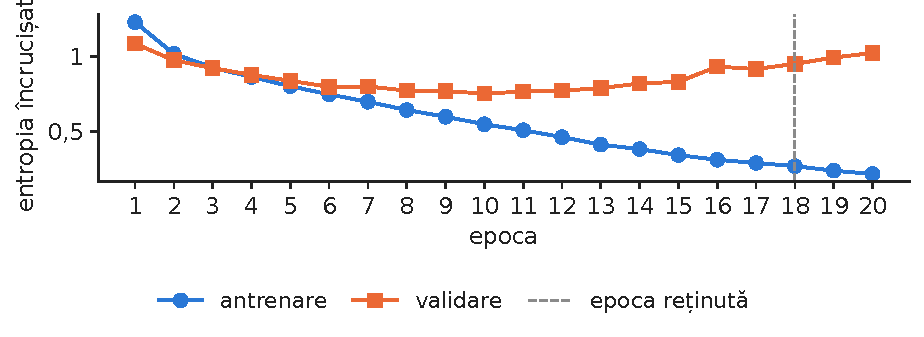
\includegraphics[width=\textwidth,height=0.500\textheight,keepaspectratio]{charts/ro/tiny_learning_curve.pdf}\end{center}\vspace{-3mm}
\chartsource{Sursa: Seturile Twitter financial news (Hugging Face, zeroshot). Date: estimări proprii; transformer mic, sămînța 1.}
\vspace{0.5mm}
\begin{itemize}\setlength{\itemsep}{0pt}
  \item \textbf{Sămînța 1}: pierderea pe validare este minimă la epoca 10 (0{,}753) și urcă la 1{,}024 pînă la epoca 20
    \begin{itemize}\setlength{\itemsep}{0pt}
      \item Macro-F1 folosit pentru oprire atinge totuși maximul la epoca 18
    \end{itemize}
  \item \textbf{Are nevoie de multe date}: 8\,588 de tweet-uri sînt puține pentru 2\,020\,547 de parametri învățați de la zero
    \begin{itemize}\setlength{\itemsep}{0pt}
      \item Modelul devine prea sigur pe el înainte să se oprească din progres
    \end{itemize}
\end{itemize}
\par\vfill\noindent{\scriptsize\color{FooterGray}}\hfill\qlink{NN\_L7\_tiny\_learning\_curve}{Quantlets/L7/NN_L7_tiny_learning_curve}\par\vspace{0.5mm}
\end{frame}

\begin{frame}{Preantrenarea cîștigă: FinBERT ajustat conduce, transformerul mic rămîne sub TF-IDF}
\small
\begin{center}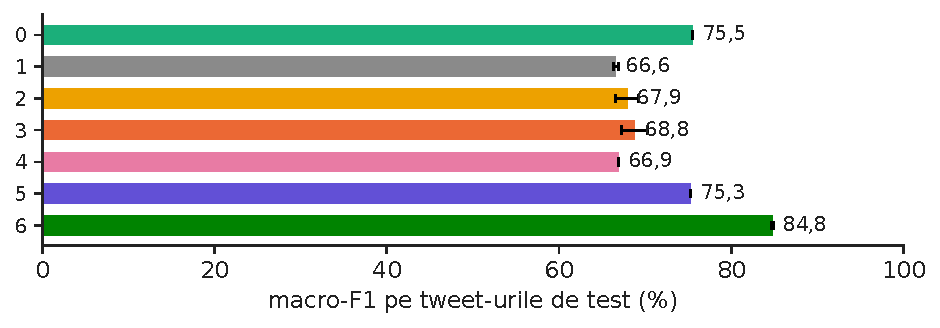
\includegraphics[width=\textwidth,height=0.449\textheight,keepaspectratio]{charts/ro/model_comparison.pdf}\end{center}\vspace{-3mm}
\chartsource{Sursa: Seturile Twitter financial news (Hugging Face, zeroshot). Date: estimări proprii; 2.388 tweet-uri de test (setul de validare publicat).}
\vspace{0.5mm}
\begin{itemize}\setlength{\itemsep}{0pt}
  \item \textbf{Macro-F1 pe 2\,388 de tweet-uri de test}: FinBERT ajustat 84{,}8\,\%, TF-IDF 75{,}5\,\%, transformerul mic 68{,}8\,\% (abatere standard 1{,}5, 3 semințe)
  \item \textbf{FinBERT fără antrenare pe tweet-uri}: 66{,}9\,\%
    \begin{itemize}\setlength{\itemsep}{0pt}
      \item FinBERT înghețat + logistic: 75{,}3\,\%
    \end{itemize}
\end{itemize}
\par\vfill\noindent{\scriptsize\color{FooterGray}}\hfill\qlink{NN\_L7\_model\_comparison}{Quantlets/L7/NN_L7_model_comparison}\par\vspace{0.5mm}
\end{frame}

\begin{frame}{Clasa negativă este cea în care modelele diferă cel mai mult}
\footnotesize
{\scriptsize\renewcommand{\arraystretch}{1.15}\setlength{\tabcolsep}{4pt}
\begin{tabular}{@{}lrrrrr@{}}\toprule
Model & Macro-F1 & Acuratețe & Recall negativ & Precizie negativ & Rulări \\ \midrule
TF-IDF + logistic & \cellcolor{Crimson!1}75{,}5 & \cellcolor{Forest!8}81{,}5 & \cellcolor{Crimson!5}70{,}3 & \cellcolor{Forest!4}63{,}5 & 1 \\
Medie embedding-uri & \cellcolor{Crimson!55}66{,}6 & \cellcolor{Crimson!43}74{,}3 & \cellcolor{Crimson!44}62{,}0 & \cellcolor{Crimson!55}46{,}6 & 3 \\
Transformer fără poziții & \cellcolor{Crimson!47}67{,}9 & \cellcolor{Crimson!35}75{,}4 & \cellcolor{Crimson!45}61{,}8 & \cellcolor{Crimson!49}48{,}4 & 3 \\
Transformer mic & \cellcolor{Crimson!42}68{,}8 & \cellcolor{Crimson!26}76{,}7 & \cellcolor{Crimson!55}59{,}7 & \cellcolor{Crimson!39}51{,}1 & 3 \\
FinBERT fără antrenare & \cellcolor{Crimson!53}66{,}9 & \cellcolor{Crimson!55}72{,}6 & \cellcolor{Forest!23}76{,}1 & \cellcolor{Crimson!45}49{,}4 & 1 \\
FinBERT înghețat + logistic & \cellcolor{Crimson!2}75{,}3 & \cellcolor{Crimson!2}80{,}1 & \cellcolor{Forest!35}78{,}7 & \cellcolor{Crimson!13}58{,}6 & 1 \\
FinBERT ajustat & \cellcolor{Forest!55}84{,}8 & \cellcolor{Forest!55}88{,}2 & \cellcolor{Forest!55}82{,}9 & \cellcolor{Forest!55}77{,}9 & 3 \\
\bottomrule\end{tabular}}
\vspace{1.5mm}
\begin{itemize}\setlength{\itemsep}{2pt}
  \item \textbf{Toate valorile în \%}, pe tweet-urile de test
    \begin{itemize}\setlength{\itemsep}{0pt}
      \item Verde = cel mai bun, roșu = cel mai slab din coloană
      \item Medii pe rulări
    \end{itemize}
  \item \textbf{Știrile negative}: FinBERT ajustat găsește 82{,}9\,\% dintre ele, cu o precizie de 77{,}9\,\%
    \begin{itemize}\setlength{\itemsep}{0pt}
      \item TF-IDF 70{,}3\,\% și 63{,}5\,\%
    \end{itemize}
\end{itemize}
\par\vfill\manager{raportați recall-ul și precizia pe clase: o medie poate ascunde un model care ratează știrile importante.}\par\vspace{0.5mm}
\par\vfill\noindent{\scriptsize\color{FooterGray}(calcule proprii)}\hfill\tryit{notebook, secțiunea 5}\par\vspace{0.5mm}
\end{frame}

\begin{frame}{Sînt diferențele reale? Bootstrap pereche pe tweet-urile de test}
\footnotesize
\intuition{Reeșantionînd tweet-urile de test, cu aceeași extragere pentru ambele modele, vedem cît s-ar putea mișca întîmplător o diferență de macro-F1.}
\begin{columns}[T,onlytextwidth]
\begin{column}{0.58\textwidth}
\[ \Delta^{*b}=F_1^{A}(\mathcal T^{*b})-F_1^{B}(\mathcal T^{*b}),\quad b=1,\dots,1000 \]\[ \text{CI}_{95\%}=[q_{0.025},q_{0.975}] \]{\footnotesize\begin{itemize}\setlength{\itemsep}{0pt}
  \item \textbf{\txtwhere}
    \begin{itemize}\setlength{\itemsep}{0pt}
      \item $\mathcal T^{*b}$ = tweet-uri de test extrase cu întoarcere
      \item $F_1$ = macro-F1 mediat pe semințele modelului
      \item Diferențe în puncte procentuale.
    \end{itemize}
\end{itemize}\par}
\end{column}
\begin{column}{0.39\textwidth}
\begin{itemize}\setlength{\itemsep}{2pt}
  \item \textbf{FinBERT ajustat $-$ TF-IDF}
    \begin{itemize}\setlength{\itemsep}{0pt}
      \item \ensuremath{+}9{,}3 [\ensuremath{+}7{,}3; \ensuremath{+}11{,}3]
    \end{itemize}
  \item \textbf{Transformer mic $-$ TF-IDF}
    \begin{itemize}\setlength{\itemsep}{0pt}
      \item \ensuremath{-}6{,}6 [\ensuremath{-}8{,}3; \ensuremath{-}4{,}9]
    \end{itemize}
  \item \textbf{Cu $-$ fără poziții}
    \begin{itemize}\setlength{\itemsep}{0pt}
      \item \ensuremath{+}0{,}9 [\ensuremath{+}0{,}1; \ensuremath{+}1{,}7]
    \end{itemize}
  \item \textbf{FinBERT înghețat $-$ TF-IDF}
    \begin{itemize}\setlength{\itemsep}{0pt}
      \item \ensuremath{-}0{,}2 [\ensuremath{-}2{,}5; \ensuremath{+}2{,}0]
    \end{itemize}
\end{itemize}
\end{column}
\end{columns}
\par\vfill\manager{un interval care nu conține zero este dovada minimă înainte de a înlocui un model aflat în producție.}\par\vspace{0.5mm}
\par\vfill\noindent{\scriptsize\color{FooterGray}(Efron \& Tibshirani, 1993)}\hfill\tryit{notebook, secțiunea 5}\par\vspace{0.5mm}
\end{frame}

\begin{frame}{Cu puține date etichetate, reprezentările preantrenate contează cel mai mult}
\small
\begin{center}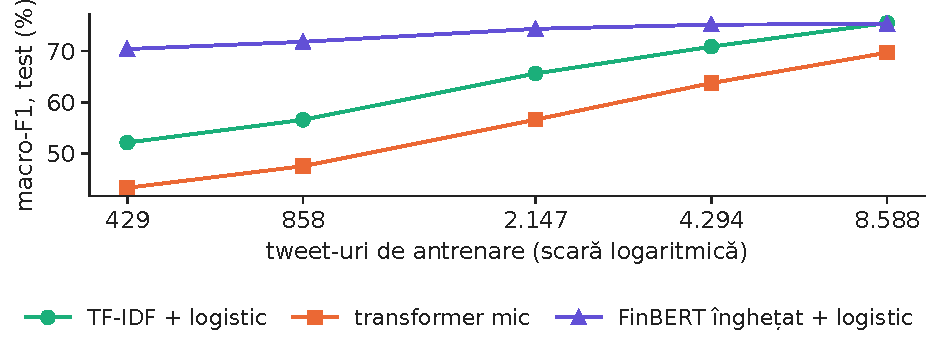
\includegraphics[width=\textwidth,height=0.464\textheight,keepaspectratio]{charts/ro/data_scaling.pdf}\end{center}\vspace{-3mm}
\chartsource{Sursa: Seturile Twitter financial news (Hugging Face, zeroshot). Date: estimări proprii; 2.388 tweet-uri de test (setul de validare publicat).}
\vspace{0.5mm}
\begin{itemize}\setlength{\itemsep}{0pt}
  \item \textbf{Cu 429 de tweet-uri de antrenare}: FinBERT înghețat + logistic 70{,}4\,\%, TF-IDF 52{,}1\,\%, transformerul mic 43{,}3\,\% macro-F1
  \item \textbf{Preantrenarea = date pe care nu le-ați etichetat}: miliarde de cuvinte au format deja vectorii FinBERT
    \begin{itemize}\setlength{\itemsep}{0pt}
      \item Un model de la zero trebuie să învețe deodată limba și sarcina
    \end{itemize}
\end{itemize}
\par\vfill\noindent{\scriptsize\color{FooterGray}(calcule proprii, sămînța 1)}\hfill\qlink{NN\_L7\_data\_scaling}{Quantlets/L7/NN_L7_data_scaling}\par\vspace{0.5mm}
\end{frame}

\begin{frame}{Ajustarea fină corectează ce greșește modelul fără antrenare}
\small
\begin{center}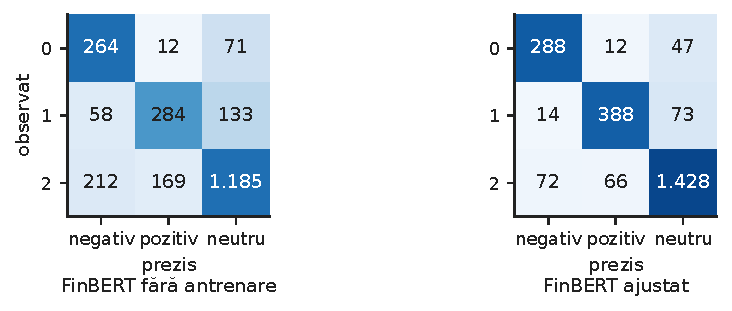
\includegraphics[width=\textwidth,height=0.479\textheight,keepaspectratio]{charts/ro/confusion.pdf}\end{center}\vspace{-3mm}
\chartsource{Sursa: Seturile Twitter financial news (Hugging Face, zeroshot). Date: estimări proprii; 2.388 tweet-uri de test (setul de validare publicat).}
\vspace{0.5mm}
\begin{itemize}\setlength{\itemsep}{0pt}
  \item \textbf{Fără antrenare}: FinBERT a fost antrenat pe propoziții din știri, nu pe tweet-uri
    \begin{itemize}\setlength{\itemsep}{0pt}
      \item Găsește 264 dintre cele 347 de tweet-uri negative
      \item După ajustare: 288
    \end{itemize}
  \item \textbf{Erorile rămase}: 47 tweet-uri negative și 73 pozitive citite ca neutre
    \begin{itemize}\setlength{\itemsep}{0pt}
      \item Doar 12 negative citite ca pozitive
    \end{itemize}
\end{itemize}
\par\vfill\noindent{\scriptsize\color{FooterGray}(calcule proprii, modelul ajustat cu sămînța 1)}\hfill\qlink{NN\_L7\_confusion}{Quantlets/L7/NN_L7_confusion}\par\vspace{0.5mm}
\end{frame}

\begin{frame}{Ajustarea fină: pornim de la ponderile preantrenate și facem pași mici}
\footnotesize
\intuition{Toate ponderile se mișcă, dar puțin: cunoștințele de limbă rămîn, stratul de decizie se adaptează la tweet-uri.}
\begin{columns}[T,onlytextwidth]
\begin{column}{0.58\textwidth}
\[ \btheta_0=\btheta_{\text{FinBERT}},\qquad \btheta_{s+1}=\btheta_s-\eta_s\,\widehat{\nabla\loss}(\btheta_s),\quad \eta_s=\eta_0\Big(1-\frac{s}{S}\Big) \]{\footnotesize\begin{itemize}\setlength{\itemsep}{0pt}
  \item \textbf{\txtwhere}
    \begin{itemize}\setlength{\itemsep}{0pt}
      \item $\eta_0=2\cdot10^{-5}$, scădere liniară pe $S$ = 3 epoci cu loturi de 32
      \item AdamW cu penalizarea ponderilor 0,01
      \item Se păstrează epoca cu cel mai bun macro-F1 pe validare.
    \end{itemize}
\end{itemize}\par}
\end{column}
\begin{column}{0.39\textwidth}
\begin{itemize}\setlength{\itemsep}{3pt}
  \item \textbf{Cîștigul}
    \begin{itemize}\setlength{\itemsep}{0pt}
      \item \ensuremath{+}17{,}9 puncte față de varianta fără antrenare, \ensuremath{+}9{,}3 față de TF-IDF
    \end{itemize}
  \item \textbf{Costul}
    \begin{itemize}\setlength{\itemsep}{0pt}
      \item 109{,}5 milioane de ponderi, 5{,}2 minute pe sămînță pe procesorul grafic al unui laptop
    \end{itemize}
  \item \textbf{Riscul}
    \begin{itemize}\setlength{\itemsep}{0pt}
      \item O rată de învățare mare șterge preantrenarea (uitare catastrofală)
    \end{itemize}
\end{itemize}
\end{column}
\end{columns}
\par\vfill\manager{ajustarea fină a unui codificator preantrenat este azi alegerea implicită pentru orice sarcină pe text etichetat, cu cîteva mii de exemple.}\par\vspace{0.5mm}
\par\vfill\noindent{\scriptsize\color{FooterGray}(Devlin et al., 2019; Araci, 2019)}\hfill\tryit{notebook, secțiunea 5}\par\vspace{0.5mm}
\end{frame}

\begin{frame}{Contează ordinea cuvintelor în tweet-uri?}
\footnotesize
\begin{columns}[T,onlytextwidth]
\begin{column}{0.49\textwidth}
\begin{itemize}\setlength{\itemsep}{5pt}
  \item \textbf{Experimentul de eliminare}
    \begin{itemize}\setlength{\itemsep}{0pt}
      \item Același transformer mic, cu și fără codificarea poziției, cîte 3 semințe
      \item Macro-F1 68{,}8\,\% cu poziții, 67{,}9\,\% fără: \ensuremath{+}0{,}9 puncte
    \end{itemize}
  \item \textbf{Bootstrap}
    \begin{itemize}\setlength{\itemsep}{0pt}
      \item Intervalul de 95\,\% al cîștigului: [\ensuremath{+}0{,}1; \ensuremath{+}1{,}7] puncte
    \end{itemize}
\end{itemize}
\end{column}
\begin{column}{0.48\textwidth}
\begin{itemize}\setlength{\itemsep}{5pt}
  \item \textbf{Interpretare}
    \begin{itemize}\setlength{\itemsep}{0pt}
      \item Tweet-urile scurte și formulaice sînt mai ales colecții de cuvinte-semnal (``cut'', ``beats'', ``downgrade'')
      \item Media de embedding-uri, fără atenție, este aproape: 66{,}6\,\%
    \end{itemize}
  \item \textbf{Cînd contează ordinea}
    \begin{itemize}\setlength{\itemsep}{0pt}
      \item Negația și contrastul (``not'', ``but''), documentele lungi, cifrele legate de entitatea corectă
    \end{itemize}
\end{itemize}
\end{column}
\end{columns}
\par\vfill\manager{testați mai întîi versiunea simplă a modelului: pe texte scurte o mare parte din puterea transformerului rămîne nefolosită.}\par\vspace{0.5mm}
\par\vfill\noindent{\scriptsize\color{FooterGray}(calcule proprii)}\hfill\tryit{notebook, secțiunea 5}\par\vspace{0.5mm}
\end{frame}


\section{Transformerele în practică}

\begin{frame}{De la scorurile de sentiment la un semnal de afaceri}
\footnotesize
\begin{columns}[T,onlytextwidth]
\begin{column}{0.49\textwidth}
\begin{itemize}\setlength{\itemsep}{5pt}
  \item \textbf{Fluxul de lucru}
    \begin{itemize}\setlength{\itemsep}{0pt}
      \item Fluxul de știri și postări $\to$ tokenizator $\to$ codificator ajustat $\to$ probabilitățile claselor
      \item Agregare pe firmă și zi: ponderea mesajelor negative minus pozitive, ponderată cu audiența
    \end{itemize}
  \item \textbf{Utilizări}
    \begin{itemize}\setlength{\itemsep}{0pt}
      \item Monitorizarea riscului unui portofoliu de credite, avertizare timpurie pentru emitenți, o intrare pentru ajustarea valorii la risc (VaR)
    \end{itemize}
\end{itemize}
\end{column}
\begin{column}{0.48\textwidth}
\begin{itemize}\setlength{\itemsep}{5pt}
  \item \textbf{Capcane}
    \begin{itemize}\setlength{\itemsep}{0pt}
      \item Informația din viitor: folosiți doar texte cu marcaj de timp anterior deciziei
      \item Schimbarea domeniului: un model pentru propoziții din știri citește greșit tweet-urile (diferența față de varianta fără antrenare)
      \item Zgomotul din etichete și sarcasmul; derivă cînd se schimbă vocabularul pieței
    \end{itemize}
\end{itemize}
\end{column}
\end{columns}
\par\vfill\manager{un scor de sentiment este o intrare într-un model, nu o decizie de tranzacționare: testați-l retrospectiv înainte de folosire.}\par\vspace{0.5mm}
\par\vfill\noindent{\scriptsize\color{FooterGray}(Tetlock, 2007)}\par\vspace{0.5mm}
\end{frame}

\begin{frame}{Documentele lungi: discursurile băncilor centrale și rapoartele anuale}
\footnotesize
\begin{columns}[T,onlytextwidth]
\begin{column}{0.49\textwidth}
\begin{itemize}\setlength{\itemsep}{5pt}
  \item \textbf{Discursurile noastre}
    \begin{itemize}\setlength{\itemsep}{0pt}
      \item 400 de discursuri ale BCE, 8 ianuarie 2022 -- 30 octombrie 2026
      \item Mediana 3\,338 de tokeni, cel mai lung 22\,646
    \end{itemize}
  \item \textbf{Costul pătratic}
    \begin{itemize}\setlength{\itemsep}{0pt}
      \item Atenția pe un discurs median costă de circa 17\,828 de ori mai mult decît pe un tweet median
    \end{itemize}
\end{itemize}
\end{column}
\begin{column}{0.48\textwidth}
\begin{itemize}\setlength{\itemsep}{5pt}
  \item \textbf{Variante}
    \begin{itemize}\setlength{\itemsep}{0pt}
      \item Împărțire în ferestre de 512 și agregarea scorurilor pe bucăți
      \item Modele ierarhice: vectori de propoziții, apoi atenție pe propoziții
      \item Modele cu context lung: atenție rară sau eficientă ca memorie
    \end{itemize}
\end{itemize}
\end{column}
\end{columns}
\par\vfill\manager{pentru o echipă de politică monetară, împărțirea în bucăți plus un codificator bine testat bate de obicei un model cu context lung netestat.}\par\vspace{0.5mm}
\par\vfill\noindent{\scriptsize\color{FooterGray}(Vaswani et al., 2017)}\hfill\tryit{notebook, secțiunea 1}\par\vspace{0.5mm}
\end{frame}

\begin{frame}{Transformerele dincolo de text}
\footnotesize
\begin{columns}[T,onlytextwidth]
\begin{column}{0.49\textwidth}
\begin{itemize}\setlength{\itemsep}{5pt}
  \item \textbf{Serii de timp}
    \begin{itemize}\setlength{\itemsep}{0pt}
      \item Fragmente ale seriei ca tokeni; modele de prognoză preantrenate (cursul 13)
    \end{itemize}
  \item \textbf{Tabele și tranzacții}
    \begin{itemize}\setlength{\itemsep}{0pt}
      \item Fiecare coloană sau fiecare plată anterioară ca token; atenție între ele
    \end{itemize}
\end{itemize}
\end{column}
\begin{column}{0.48\textwidth}
\begin{itemize}\setlength{\itemsep}{5pt}
  \item \textbf{Grafuri}
    \begin{itemize}\setlength{\itemsep}{0pt}
      \item Atenția restrînsă la muchii = rețeaua cu atenție pe graf (cursul 9)
    \end{itemize}
  \item \textbf{Imagini și documente}
    \begin{itemize}\setlength{\itemsep}{0pt}
      \item Fragmente de imagine ca tokeni; modelele viziune-limbaj citesc grafice și rapoarte (cursul 14)
    \end{itemize}
\end{itemize}
\end{column}
\end{columns}
\par\vfill\manager{oricare ar fi datele, întrebarea este aceeași: care sînt tokenii și ce perechi au voie să-și acorde atenție?}\par\vspace{0.5mm}
\par\vfill\noindent{\scriptsize\color{FooterGray}(Bishop \& Bishop, 2024, ch.\ 12)}\par\vspace{0.5mm}
\end{frame}


\section{Concluzii}

\begin{frame}{Ce reținem}
\small
\begin{itemize}\setlength{\itemsep}{6pt}
  \item \textbf{Atenția} = softmax al scorurilor întrebare-cheie scalate, înmulțit cu valorile
    \begin{itemize}\setlength{\itemsep}{0pt}
      \item Un singur pas între oricare două cuvinte, cost $O(n^2)$
      \item $\sqrt{d_k}$ păstrează softmax-ul antrenabil
    \end{itemize}
  \item \textbf{Blocul transformer} = atenție cu mai multe capete + rețea directă, fiecare cu conexiune reziduală și normalizare
    \begin{itemize}\setlength{\itemsep}{0pt}
      \item Pozițiile se adaugă, pentru că atenția ignoră ordinea
    \end{itemize}
  \item \textbf{Pe tweet-urile financiare} preantrenarea decide: FinBERT ajustat 84{,}8\,\% macro-F1, TF-IDF 75{,}5\,\%, un transformer de la zero 68{,}8\,\%
  \item \textbf{Hărțile de atenție} sînt indicii, nu explicații
    \begin{itemize}\setlength{\itemsep}{0pt}
      \item Verificați erorile pe clase și intervalele bootstrap înainte de a avea încredere într-un model
    \end{itemize}
\end{itemize}
\end{frame}

\begin{frame}{Cercetările grupului nostru: transformerele ca instrumente de prognoză a riscului}
\footnotesize
\begin{itemize}\setlength{\itemsep}{5pt}
  \item \textbf{Modele mari de limbaj (LLM) pentru prognoza riscului extrem} (Pele, Bolovăneanu, Lin, Ren, Ginavar, Spilak, Andrei, Toma, Lessmann \& Härdle, 2026)
    \begin{itemize}\setlength{\itemsep}{0pt}
      \item Lucrarea folosește transformere decodor, cărora li se dau istoricele randamentelor, pentru prognoza valorii la risc și a pierderii așteptate în coadă (ES) --- LLM-VaR și LLM-ES --- și le evaluează cu testele retrospective standard
    \end{itemize}
  \item \textbf{Modele fundaționale pentru riscul extrem} (Jheng, Tak, Găman, Mazurencu-Marinescu-Pele \& Pele, 2026)
    \begin{itemize}\setlength{\itemsep}{0pt}
      \item Lucrarea folosește modele transformer de prognoză preantrenate, fără reantrenare și cu calibrare conformală, pentru prognoza VaR și ES pe piețele din Europa Centrală și de Est
    \end{itemize}
  \item \textbf{Legătura cu acest curs}: aceeași idee ca la FinBERT, un model preantrenat pe date multe și folosit cu puțină sau fără antrenare specifică, aplicată măsurilor de risc în loc de cuvinte
\end{itemize}
\vspace{1mm}{\scriptsize Rezultatele de pe acest slide sînt cele din lucrări; cifrele de pe celelalte slide-uri provin din calculele noastre.}
\par\vfill\noindent{\scriptsize\color{FooterGray}(Academia de Studii Economice din București; Academia Română, Institutul de Prognoză Economică)}\par\vspace{0.5mm}
\end{frame}

\begin{frame}{Lecturi și resurse suplimentare}
\small
\begin{columns}[T,onlytextwidth]
\begin{column}{0.52\textwidth}
\begin{itemize}\setlength{\itemsep}{4pt}
  \item \textbf{Vaswani et al.\ (2017)}, ``Attention is all you need'': transformerul original
  \item \textbf{Bishop \& Bishop (2024)}, capitolul 12: transformerele, de la atenție la modelele mari de limbaj
  \item \textbf{The Illustrated Transformer} (J.\ Alammar): \href{https://jalammar.github.io/illustrated-transformer/}{jalammar.github.io}.
\end{itemize}
\end{column}
\begin{column}{0.45\textwidth}
\begin{itemize}\setlength{\itemsep}{4pt}
  \item \textbf{Cursul Hugging Face}, ajustarea codificatoarelor: \href{https://huggingface.co/learn/llm-course}{huggingface.co/learn}.
  \item \textbf{Acest curs}: cod, date, notebook-uri --- \href{https://github.com/danpele/NEURAL_BIZ}{github.com/danpele/NEURAL\_BIZ}.
  \item \textbf{Exercițiu practic}: notebook-ul reproduce toate graficele și cifrele acestui curs
\end{itemize}
\end{column}
\end{columns}
\end{frame}

\begin{frame}{Test 1: scalarea}
\small
\begin{itemize}
  \item De ce se împart scorurile de atenție la $\sqrt{d_k}$?
\end{itemize}
\vspace{2mm}
\begin{exampleblock}{R\u{a}spuns}
\begin{itemize}
  \item Cu elemente de varianță unu, produsul scalar $\mathbf q^{\top}\mathbf k$ are varianța $d_k$
    \begin{itemize}\setlength{\itemsep}{0pt}
      \item Împărțirea la $\sqrt{d_k}$ o readuce la 1, deci softmax-ul nu se saturează și gradientul nu dispare
    \end{itemize}
\end{itemize}
\end{exampleblock}
\end{frame}

\begin{frame}{Test 2: pozițiile}
\small
\begin{itemize}
  \item Ce se întîmplă cu un transformer fără codificarea poziției?
\end{itemize}
\vspace{2mm}
\begin{exampleblock}{R\u{a}spuns}
\begin{itemize}
  \item Auto-atenția este echivariantă la permutări, deci modelul vede o colecție de tokeni
    \begin{itemize}\setlength{\itemsep}{0pt}
      \item Pe tweet-urile noastre scurte costul a fost doar 0{,}9 puncte de macro-F1, dar ordinea contează pentru negație și texte lungi
    \end{itemize}
\end{itemize}
\end{exampleblock}
\end{frame}

\begin{frame}{Test 3: preantrenarea}
\small
\begin{itemize}
  \item De ce pierde în fața TF-IDF un transformer antrenat de la zero pe 8\,588 de tweet-uri?
\end{itemize}
\vspace{2mm}
\begin{exampleblock}{R\u{a}spuns}
\begin{itemize}
  \item Trebuie să învețe limba și sarcina din puține exemple, cu 2\,020\,547 de parametri
    \begin{itemize}\setlength{\itemsep}{0pt}
      \item FinBERT preantrenat aduce aceste cunoștințe și ajunge la 84{,}8\,\% după ajustare
    \end{itemize}
\end{itemize}
\end{exampleblock}
\end{frame}

\begin{frame}{Test 4: codificator sau decodor}
\small
\begin{itemize}
  \item O bancă vrea să eticheteze după subiect 10.000 de reclamații pe zi.
    \begin{itemize}\setlength{\itemsep}{0pt}
      \item Transformer codificator sau decodor?
    \end{itemize}
\end{itemize}
\vspace{2mm}
\begin{exampleblock}{R\u{a}spuns}
\begin{itemize}
  \item Un codificator (de tip BERT), ajustat pe reclamații etichetate: citește tot textul în ambele direcții și produce probabilitățile claselor, ieftin și consecvent
\end{itemize}
\end{exampleblock}
\end{frame}

\begin{frame}{Test 5: hărțile de atenție}
\small
\begin{itemize}
  \item Poate o hartă de atenție să justifice o decizie în fața unui supraveghetor?
\end{itemize}
\vspace{2mm}
\begin{exampleblock}{R\u{a}spuns}
\begin{itemize}
  \item Nu: hărți diferite pot da aceeași predicție, iar multă atenție merge spre [SEP] (pînă la 59{,}3\,\% aici)
    \begin{itemize}\setlength{\itemsep}{0pt}
      \item Se folosesc metode de atribuire și teste
    \end{itemize}
\end{itemize}
\end{exampleblock}
\end{frame}

\begin{frame}{Bibliografie (1/2)}
\scriptsize
\begin{itemize}\setlength{\itemsep}{0pt}\scriptsize
\item Araci, D.\ (2019). FinBERT: Financial sentiment analysis with pre-trained language models. \href{https://arxiv.org/abs/1908.10063}{arXiv:1908.10063}
\item Ba, J.\,L., Kiros, J.\,R.\ \& Hinton, G.\,E.\ (2016). Layer normalization. \href{https://arxiv.org/abs/1607.06450}{arXiv:1607.06450}
\item Bahdanau, D., Cho, K.\ \& Bengio, Y.\ (2015). Neural machine translation by jointly learning to align and translate. \textit{International Conference on Learning Representations}. \href{https://arxiv.org/abs/1409.0473}{arXiv:1409.0473}
\item Bishop, C.\,M.\ \& Bishop, H.\ (2024). \textit{Deep Learning: Foundations and Concepts}, ch.\ 12. Springer. \href{https://doi.org/10.1007/978-3-031-45468-4}{doi:10.1007/978-3-031-45468-4}
\item Clark, K., Khandelwal, U., Levy, O.\ \& Manning, C.\,D.\ (2019). What does BERT look at? An analysis of BERT's attention. \textit{BlackboxNLP Workshop}, 276--286. \href{https://doi.org/10.18653/v1/W19-4828}{doi:10.18653/v1/W19-4828}
\item Devlin, J., Chang, M.-W., Lee, K.\ \& Toutanova, K.\ (2019). BERT: Pre-training of deep bidirectional transformers for language understanding. \textit{Proceedings of NAACL}, 4171--4186. \href{https://doi.org/10.18653/v1/N19-1423}{doi:10.18653/v1/N19-1423}
\item Efron, B.\ \& Tibshirani, R.\,J.\ (1993). \textit{An Introduction to the Bootstrap}. Chapman \& Hall. \href{https://doi.org/10.1201/9780429246593}{doi:10.1201/9780429246593}
\item Jain, S.\ \& Wallace, B.\,C.\ (2019). Attention is not explanation. \textit{Proceedings of NAACL}, 3543--3556. \href{https://doi.org/10.18653/v1/N19-1357}{doi:10.18653/v1/N19-1357}
\end{itemize}
\end{frame}

\begin{frame}{Bibliografie (2/2)}
\scriptsize
\begin{itemize}\setlength{\itemsep}{0pt}\scriptsize
\item Jheng, S.-L., Tak, R., Găman, Ș., Mazurencu-Marinescu-Pele, M.\ \& Pele, D.\,T.\ (2026). Can foundation models manage risk? Zero-shot VaR and ES forecasting with conformal calibration in CEE markets. \textit{Economic Computation and Economic Cybernetics Studies and Research}, 60(2), 267--290. \href{https://doi.org/10.24818/18423264/60.2.26.14}{doi:10.24818/18423264/60.2.26.14}
\item Loshchilov, I.\ \& Hutter, F.\ (2019). Decoupled weight decay regularization. \textit{International Conference on Learning Representations}. \href{https://arxiv.org/abs/1711.05101}{arXiv:1711.05101}
\item Malo, P., Sinha, A., Korhonen, P., Wallenius, J.\ \& Takala, P.\ (2014). Good debt or bad debt: Detecting semantic orientations in economic texts. \textit{Journal of the Association for Information Science and Technology}, 65(4), 782--796. \href{https://doi.org/10.1002/asi.23062}{doi:10.1002/asi.23062}
\item Pele, D.\,T., Bolovăneanu, V., Lin, M.-B., Ren, R., Ginavar, A.\,T., Spilak, B., Andrei, A.-V., Toma, F.-M., Lessmann, S.\ \& Härdle, W.\,K.\ (2026). In the beginning was the word: LLM-VaR and LLM-ES. SSRN Working Paper 5104383. \href{https://doi.org/10.2139/ssrn.5104383}{doi:10.2139/ssrn.5104383}
\item Radford, A., Narasimhan, K., Salimans, T.\ \& Sutskever, I.\ (2018). Improving language understanding by generative pre-training. OpenAI technical report. \href{https://openai.com/research/language-unsupervised}{openai.com/research/language-unsupervised}
\item Tetlock, P.\,C.\ (2007). Giving content to investor sentiment: The role of media in the stock market. \textit{Journal of Finance}, 62(3), 1139--1168. \href{https://doi.org/10.1111/j.1540-6261.2007.01232.x}{doi:10.1111/j.1540-6261.2007.01232.x}
\item Vaswani, A., Shazeer, N., Parmar, N., Uszkoreit, J., Jones, L., Gomez, A.\,N., Kaiser, Ł.\ \& Polosukhin, I.\ (2017). Attention is all you need. \textit{Advances in Neural Information Processing Systems}, 30. \href{https://arxiv.org/abs/1706.03762}{arXiv:1706.03762}
\item Wu, Y., Schuster, M., Chen, Z.\ et al.\ (2016). Google's neural machine translation system: Bridging the gap between human and machine translation. \href{https://arxiv.org/abs/1609.08144}{arXiv:1609.08144}
\end{itemize}
\end{frame}

\appendix

\section*{Anexă}

\begin{frame}{Anexa A: gradientul softmax-ului și saturația}
\small
\begin{columns}[T,onlytextwidth]
\begin{column}{0.50\textwidth}
\[ a_j=\frac{e^{s_j}}{\sum_l e^{s_l}},\qquad \frac{\partial a_j}{\partial s_i}=a_j(\delta_{ij}-a_i) \]\[ J=\operatorname{diag}(\mathbf a)-\mathbf a\mathbf a^{\top},\qquad \|J\|\to0\ \text{cînd}\ \mathbf a\to\mathbf e_k \]
\end{column}
\begin{column}{0.47\textwidth}
\begin{itemize}\setlength{\itemsep}{3pt}
  \item Dacă un scor domină, $\mathbf a$ este aproape one-hot și toate elementele lui $J$ sînt aproape zero: întrebările și cheile nu mai învață
  \item Scorurile cu abaterea standard $\sigma$ fac dominarea probabilă cînd $\sigma$ este mare
    \begin{itemize}\setlength{\itemsep}{0pt}
      \item Scalarea cu $\sqrt{d_k}$ fixează $\sigma=1$ la inițializare
    \end{itemize}
\end{itemize}
\end{column}
\end{columns}
\par\vfill\noindent{\scriptsize\color{FooterGray}(Vaswani et al., 2017)}\par\vspace{0.5mm}
\end{frame}

\begin{frame}{Anexa B: parametrii unui bloc transformer}
\small
\begin{columns}[T,onlytextwidth]
\begin{column}{0.50\textwidth}
\[ \underbrace{4d^2+4d}_{\text{atenție}}+\underbrace{8d^2+5d}_{\text{FFN}}+\underbrace{4d}_{\text{LN}}\ \approx\ 12d^2 \]
\end{column}
\begin{column}{0.47\textwidth}
\begin{itemize}\setlength{\itemsep}{3pt}
  \item Atenția: $W_Q,W_K,W_V,W_O\in\R^{d\times d}$, cu termeni liberi
    \begin{itemize}\setlength{\itemsep}{0pt}
      \item FFN: $W_1\in\R^{4d\times d}$, $W_2\in\R^{d\times4d}$
      \item Două normalizări cu $\boldsymbol\gamma,\boldsymbol\beta$
    \end{itemize}
  \item BERT-base, $d=768$: circa 7 milioane pe bloc, 85 de milioane în 12 blocuri, plus 23 de milioane în tabelul reprezentărilor (după datele publicate)
\end{itemize}
\end{column}
\end{columns}
\par\vfill\noindent{\scriptsize\color{FooterGray}(Devlin et al., 2019)}\par\vspace{0.5mm}
\end{frame}

\begin{frame}{Anexa C: setările experimentelor}
\small
{\scriptsize\renewcommand{\arraystretch}{1.05}\setlength{\tabcolsep}{4pt}
\begin{tabular}{@{}p{0.27\textwidth}p{0.66\textwidth}@{}}\toprule
Model & Setări \\ \midrule
TF-IDF & secvențe de 1--2 cuvinte, minimum 2 documente, frecvență sublineară; regresie logistică cu ponderi de clasă echilibrate, $C$ = 3 ales pe validare \\
Transformer mic & tokenii WordPiece ai FinBERT, 64 de tokeni; $d=64$, 4 capete, 2 blocuri cu normalizare înainte, FFN 128, dropout 0,1; AdamW $5\cdot10^{-4}$, lot 64, cel mult 20 de epoci, răbdare 4 \\
FinBERT ajustat & versiunea ProsusAI, cu stratul de 3 clase reasociat claselor negativ/pozitiv/neutru; AdamW $2\cdot10^{-5}$, scădere liniară, lot 32, 3 epoci; semințele 1--3 \\
FinBERT înghețat & media ultimului strat ascuns pe tokenii reali; regresie logistică, $C$ = 0{,}03 \\
Echipament & laptop cu procesor Apple, procesorul grafic, Metal Performance Shaders (MPS); rularea completă 8{,}1 minute \\
\bottomrule\end{tabular}}
\end{frame}

\end{document}
